\chapter{Detail study of $\Upsilon$ suppression in Pb+Pb collisions using 150 $\mu$b$^{-1}$ data with CMS detector at LHC.} 
\label{chap:UpsilonProductionPbPb2011}

\section{Introduction}
\label{sec:introduction}
%I modify.
The LHC allows for the first detailed studies of the bottomonium family of states in ultra-relativistic 
heavy-ion collisions. Given the momentum resolution attained, and the capability of the trigger system,  
CMS is well positioned to lead these studies. The measurement of bottomonium production and suppression is 
presented, based on the dataset collected by the CMS experiment during the 2011 PbPb collision run at  $\sqrtsnn = 2.76\TeV$. 

If a deconfined medium is formed in high-energy heavy-ion collisions, one of its most striking expected characteristics is the 
suppression of quarkonium states~\cite{Matsui:1986dk}. 
This takes place as the force between the constituents of the quarkonium state, a heavy quark and its antiquark, is weakened by 
the color screening produced by the surrounding light quarks and gluons.
The suppression is predicted to occur above a critical temperature of the medium, and sequentially, in the
order of the \QQbar binding energy. 
Since the \PgUa is the most tightly bound state among all quarkonia, it is expected to be the one
with the highest dissociation temperature. % in the QGP.
Such a suppression pattern is expected to further depend on complications arising from additional phenomena sometimes referred to as
$hot$ and $cold$ nuclear matter effects~\cite{Brambilla:2010cs,Vogt:2010aa}. 
%
The study of charmonium (\Jpsi, $\psi'$, $\chi_c$) and bottomonium ($\PgUa, \PgUb, \PgUc$, $\chi_b$) production at the unprecedented medium 
created at the LHC is accordingly much awaited.  
In this chapter, the measurements of the production and suppression of the $\PgUa$,  $\PgUb$, and  $\PgUc$ states are performed. 
The production of $\PgU$(nS) states is studied by comparing their production rates in PbPb and pp collision data, taken at the same collision 
energy of $\sqrt{s_{NN}}=2.76\,\TeV$.
In particular, the yield of the higher-mass states is measured relative to the ground state. In this way, we explore the double ratios  
--  $\PgU(2S,3S)~vs~\PgUa$ and \PbPb~$vs~\pp$ --which allows a self-calibrating measurement.  
%
Several effects associated to selection, acceptance, and reconstruction mostly cancel, and only remaining factors need to be accounted for,  
as corrections to the fitted ratio of raw signal yields.  
Based on the dataset collected during the first LHC PbPb run, at $\sqrtsnn = 2.76\TeV$, in 2010, and in the special $\Pp\Pp$ run at the 
same energy in early 2011, CMS has published first results on upsilon production and suppression in PbPb collisions. 
%
These included the first evidence for suppression of the excited $\PgU$ states relative to the ground state, at the $2.4\,\sigma$ level as 
discussed in chapter\ref{chap:UpsilonProductionPbPb2010}.%~\cite{prl,QM2011}. 
Suppression of the $\PgUa$ state, relative to $\Pp\Pp$ collisions at the same energy, has also been measured~\cite{prl,QM2011}. 
These two measurements were found to be consistent with suppression of only the excited states, which result in reduced feeddown 
from excited to ground states. These main results may be summarized as follows:
%
\begin{linenomath}
\begin{eqnarray}
  \PgU(2S+3S)/\PgUa|_{\PbPb} & = & 0.24 _{-0.12}^{+0.13} \pm 0.02\,, \nonumber \\
  \PgU(2S+3S)/\PgUa|_{\pp} & = & 0.78 _{-0.14}^{+0.16} \pm 0.02\,,  \nonumber \\
(\chi \equiv)
  \frac{\PgU(2S+3S)/\PgUa|_{\PbPb}}{\PgU(2S+3S)/\PgUa|_{\pp}}
 & = & 0.31 _{-0.15}^{+0.19} \pm 0.03 \,,  \nonumber \\
(\raa \equiv)
 \frac{\PgUa|_{\PbPb;\, 0-20\%}}{\PgUa|_{\pp}}
& = & 0.681 \pm 0.143 \pm 0.119 \,.  \nonumber
%\label{eq:intro-rat}
\end{eqnarray}
\end{linenomath}
In the 2011 PbPb run, CMS collected a dataset approximately 20 times larger than that gathered in 2010. 
These data will be scrutinized, in order to extract further novel and precision results, during the 
few years ensuing datataking.
In what follows, the corresponding analysis of upsilon suppression is detailed.


\section{Data Selection}
\label{sec:dataselection}
The data analysis starts with the Onia2MuMu skim which contains all pairs of global muons with an invariant mass larger than 2 \GeVc. 
All charge combinations are considered and all possible combinations within an event are kept.
The package that was used for the skimming can be found in CVS under CMSSW/HeavyFlavorAnalysis/Onia2MuMu.
Starting from this skim a TTree is filled with single muons and muon pairs that pass quality
criteria to reject the background of fake muons while keeping the efficiency of selecting real muons high.

In order to select good quality muons, different variables were studied. This section describes how the cuts are defined and what is 
the final set of quality criteria that used in the analysis. These might not be very important for a ratio analysis but it is also a 
preparation for a more detailed analysis of the nuclear modification factor.

Muon candidates are selected if reconstructed as \emph{global muons}. Muon arbitration requirements are applied, 
specifically muons must be both global and tracker muons (accessed via the standard methods {\tt{isGlobal()}} and {\tt{isTracker()}}). 
Muon candidates are accepted if belonging to the kinematic region given by 
%
\begin{linenomath}
\begin{equation}
|\eta^\mu|<2.4 \quad \text{and} \quad \pt^\mu>4.0 \GeVc \,.
\label{eqn:muon_acc}
\end{equation}
\end{linenomath}
%
where the single muon \pt cut was determined with the optimization procedure described below.
This region is within acceptance for muon reconstruction. The optimal muon \pt threshold for the analysis is 
investigated in Sec.~\ref{sec:shoulder}.

\subsection{Optimization procedure}
The leading figure of merit employed in the optimization study is the $\PgUa$ {peak significance}, ${\cal{S}}$, defined as
%
\begin{linenomath}
\begin{equation}
{\cal{S}} \equiv \frac{N_\text{signal}}{\sqrt{N_\text{signal}+N_\text{background}}} \,,
\label{eqn:peak_signif}
\end{equation}
\end{linenomath}
%
where $N_\text{signal}$ and $N_\text{background}$ are the $\PgUa$ signal and background yields, respectively, estimated in a $\pm 100 \MeVcc$ signal window around the $\PgUa$ peak. 
Each variable will be studied for dimuons falling in the $\PgU$ mass range $\in[7, 14] \GeVcc$. 
The signal yields are obtained from the Monte Carlo sample.  by counting the dimuons in the $[-0.1, 0.1] \GeVcc$ signal window around the $\PgUa$ peak. 
%The background yields are estimated from the data sidebands using two 1 \GeVcc wide intervals placed symmetrically around the $\PgUa$ peak. 
The background yields are estimated from the data in the signal window around the $\PgUa$ peak. 
%The starting signal/background level is set from a fit to the data obtained with default cuts. 
%For estimating the background, we fit in the sidebands with a first order polynomial and extract its level from the integral of the fit in the signal window.
%
It is important to note that using the significance on data to check the effect of a cut on the signal and background could lead to a bias in the results if 
one would try to optimize the signal only looking at the data. This is why a careful attention was made to only use the significance as an indicator of the impact of the background 
rejection. We always associated the significance value with the efficiency estimation based on the MC sample.
The samples used include:
\begin{itemize}
\item realistic \PgU embedded in HYDJET \PbPb background: where the signal efficiency can be studied with the caveat that because one signal is embedded per minimum bias event, 
the signal over background ratio is greatly over-estimated;
\item prompt reconstruction of the data: where the background rejection can be studied   
\end{itemize}

\subsection{Track and dimuon quality}

The following quantities are studied:
\begin{itemize}
\item the number of valid hits within the pixels and the strips (inner tracker) a single muon track has, indicating how good the inner track part of the track is;
\item the number of pixel layers, with valid hits, crossed by a single muon. There are 2-3\% of muons with tracks with 0 pixel hit;
\item the $\chi^2/\text{ndf}$ of the single muon inner track, which indicates the quality of the inner track fit;
\item the $\chi^2/\text{ndf}$ of the single muon global track, which indicates the quality of the global fit;
\item the number of muon valid hits 
\item the distance between the event vertex and the muon track in the transverse plane, $D_{xy}$, and the longitudinal plane, $D_z$, which indicates if the muon comes from
 a decay in flight or is a prompt muon, and removes cosmics;
\item the probability of two tracks to belong to the same decay vertex.
\end{itemize}
In addition to the significance ${\cal{S}}$, the following factors are also estimated: 
(i)the efficiency of the signal using the MC sample, defined as the signal fraction measured after applying the cut, relative the number of signal events found before applying the cut; and 
(ii)the background rejection, 
defined as one minus the background fraction estimated after applying the cut, relative to the background yield estimated without the cut.
These estimators are evaluated for each variable, applying all other cuts, as a function of the cut threshold value. 
This is an iterative process, where the standard thresholds of Ref.~\cite{CMS_AN_2011_062} are used as a first iteration step. 
The procedure is applied to several track quality criteria. The aim is to confirm the goodness of the standard thresholds applied, and identify potential gains in significance that could be 
attained by adjusting the threshold of some of the inspected variables. In general, when only marginal significance improvements would be obtained, we opt to conservatively retain the initial 
standard cut thresholds; this is true in particular for those variables which could be affected by possible mismatches between data and simulation. 
Figures~\ref{fig:mu_inner_track_hit}--\ref{fig:mu_vprob} show, for each variable, the variation of the significance ${\cal{S}}$, on the left.  %on the data 
On the right hand side,  the signal efficiency and background rejection, % on MC, this for different value of the cut. 
as a functions of the probed cut value, are also displayed. 
For all variables but the one being studied, the default values are applied. 
In general, the cut chosen is the one that keeps as much signal as possible on the MC with a relatively good significance. For all plots the background rejection behaves similarly 
(but symmetrically) to the efficiency. This suggests that the background is mostly made of real tracks and/or muons, and thus difficult to reduce.
Figure~\ref{fig:mu_inner_track_hit} shows that, for the inner track number of valid hits, the significance starts dropping when more than 13 valid hits for the muon inner track is required on 
the data and the efficiency at 12. The cut chosen is mu\_innerTrack\_Hits$>$10.
%
\begin{figure}[h!]
 \begin{center}
   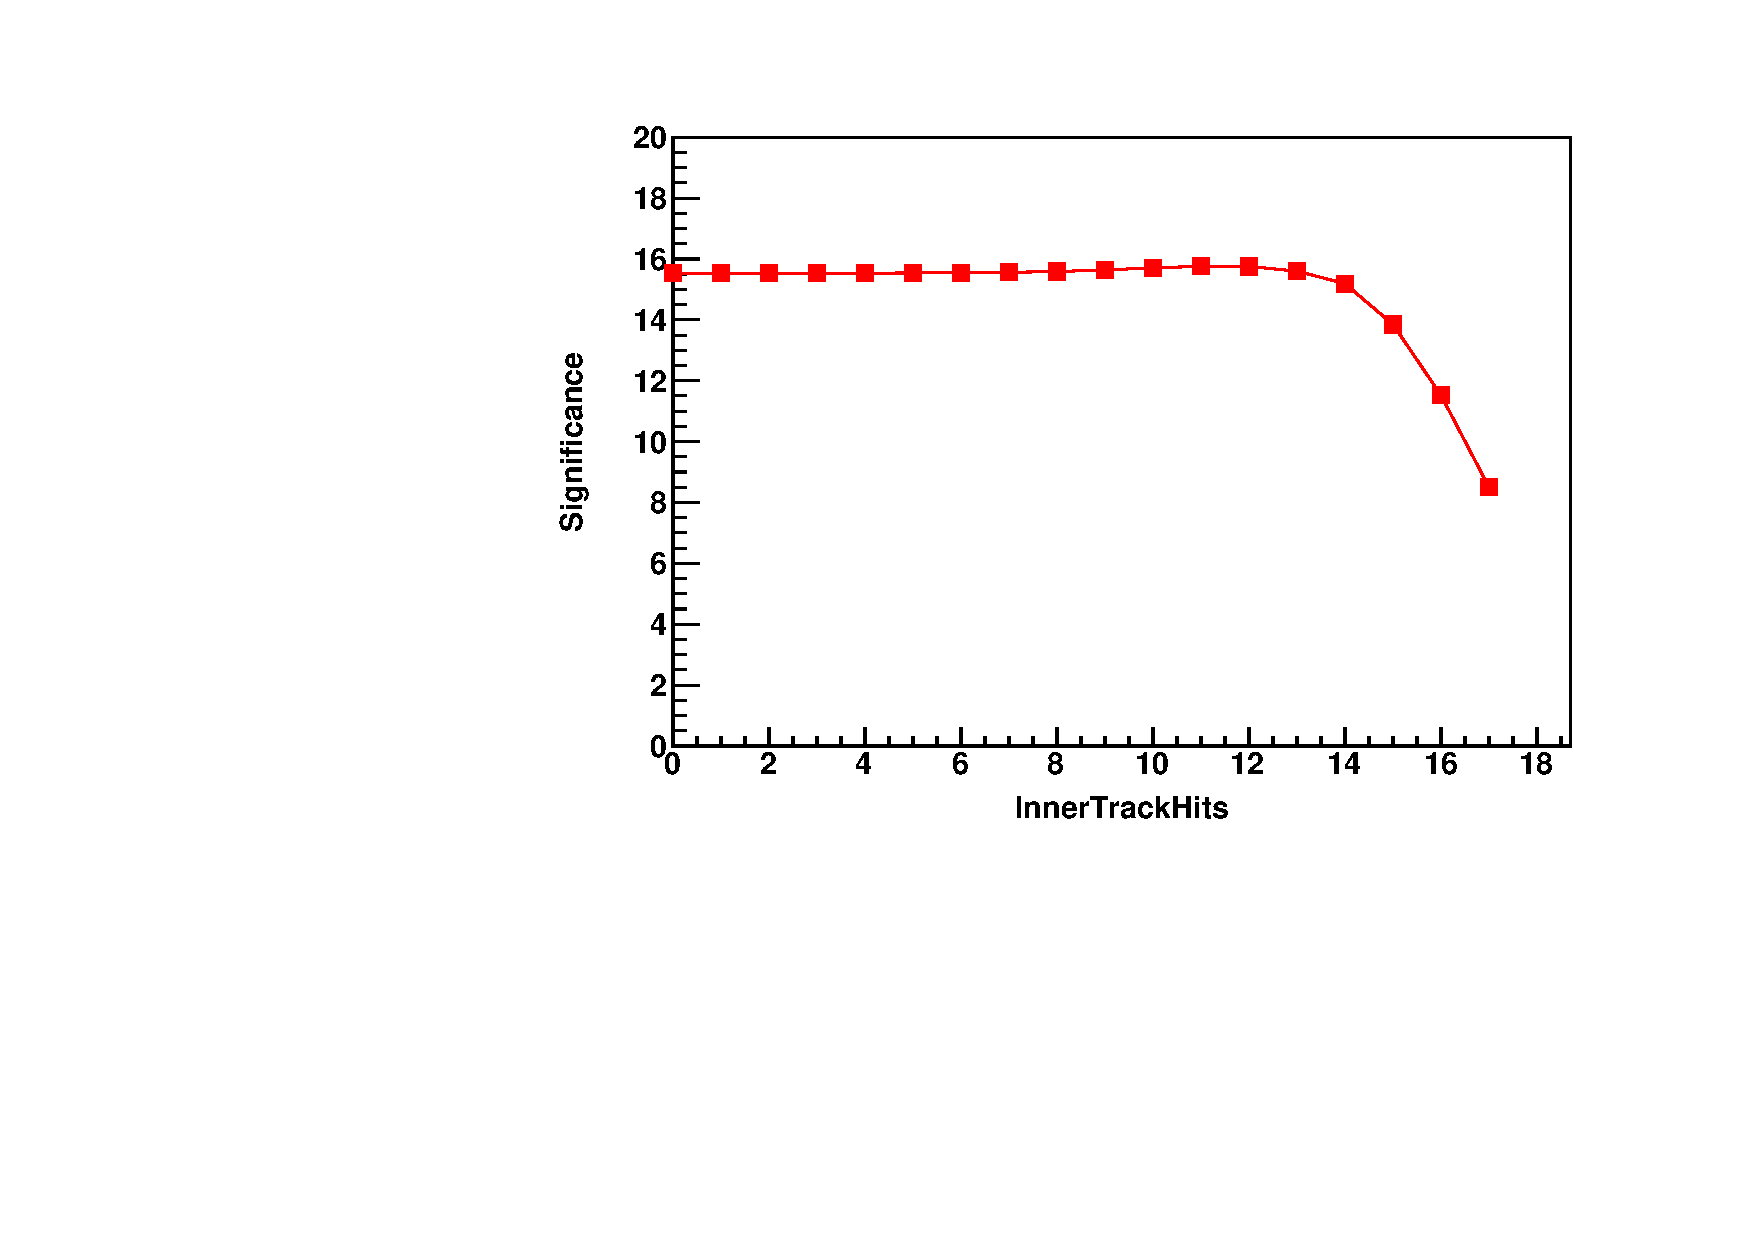
\includegraphics[angle=0,width=0.45\textwidth]{chap_YInPbPbColl2011_figures/InTrackHits_Significance1} 
   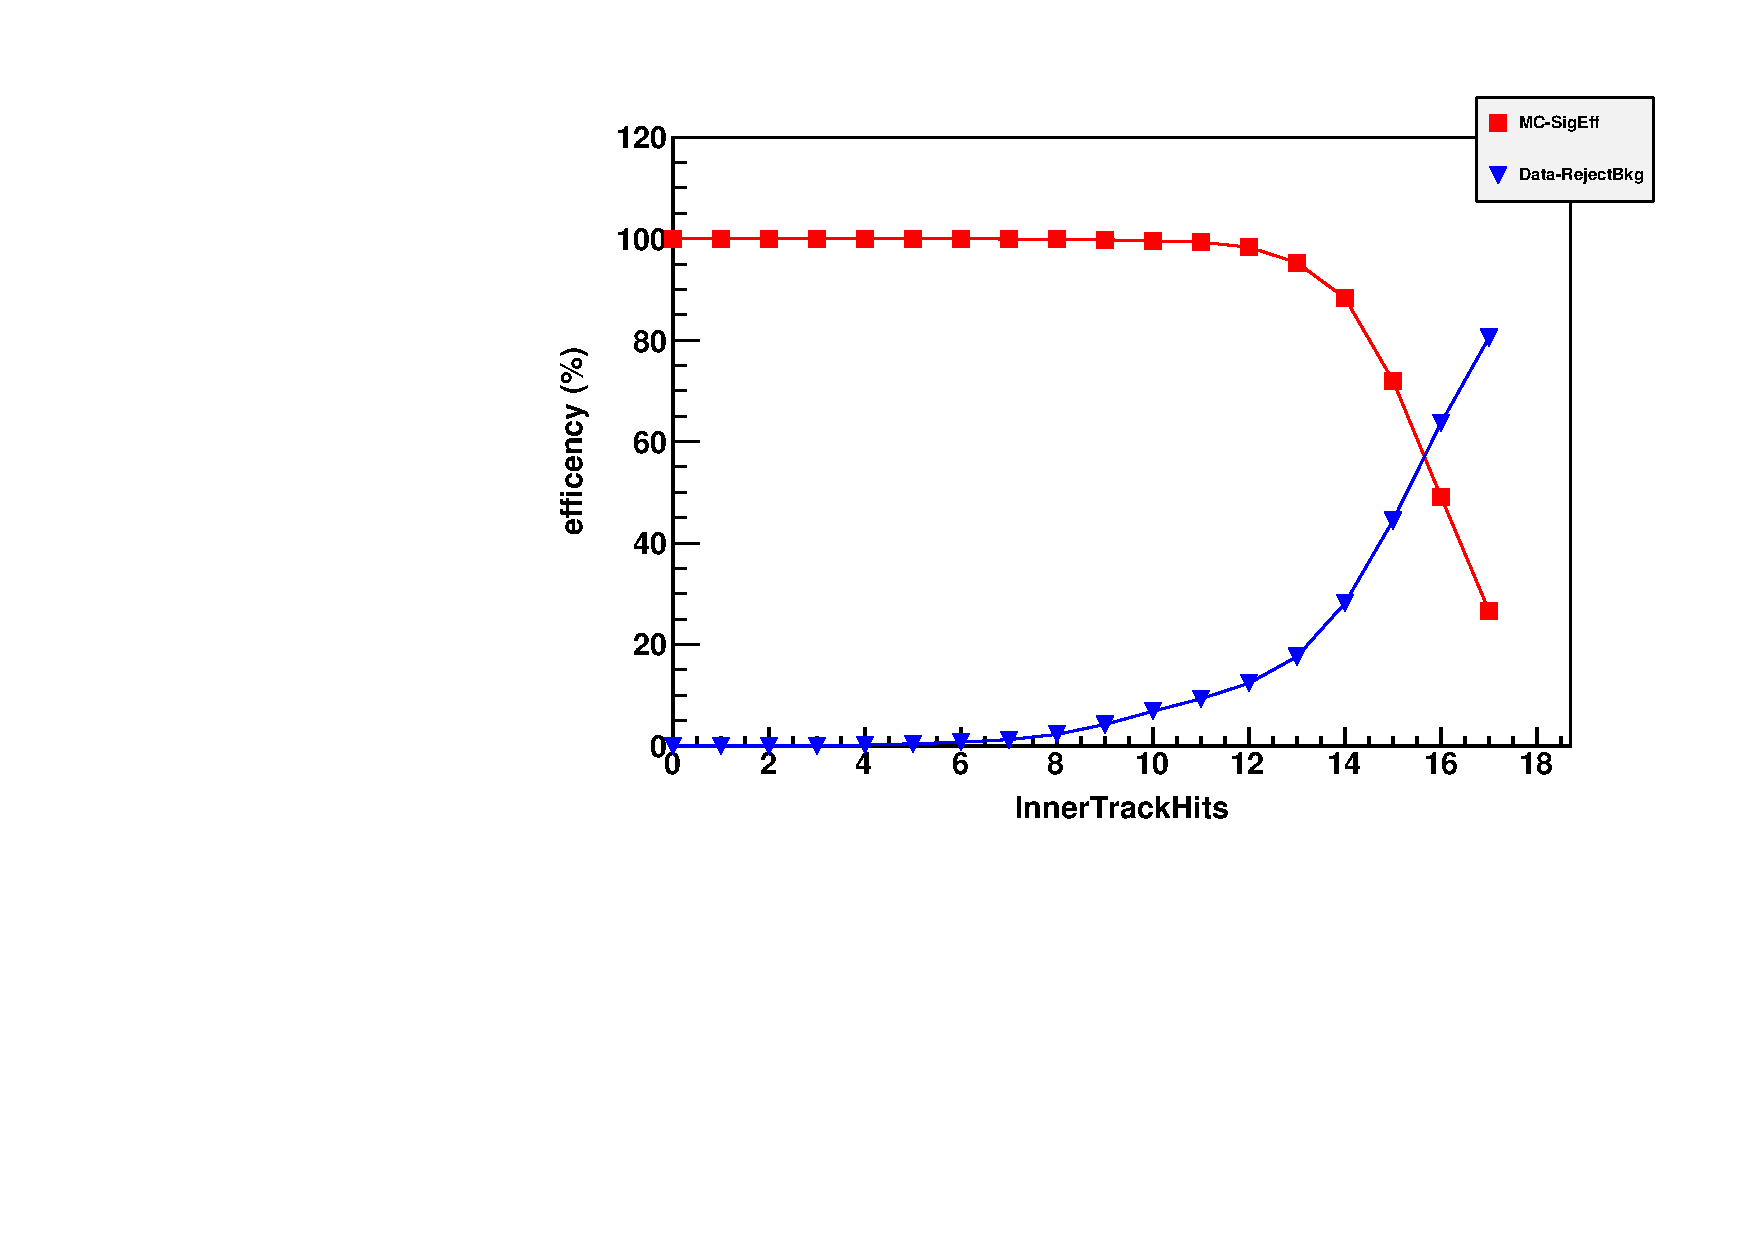
\includegraphics[angle=0,width=0.45\textwidth]{chap_YInPbPbColl2011_figures/InTrackHits_SigBkgRejEff}
   \caption{Number of muon inner track valid cut study (default: $>10$).}
   \label{fig:mu_inner_track_hit}
 \end{center}
\end{figure}

Figure~\ref{fig:mu_pixelLayers} shows that for the number of pixel layers, with valid hits, crossed, the significance 
and the efficiency are flat for 1 or 2 but there is a slight efficiency drop with the requirement of 3 pixel layers to be fulfilled, 
as does the significance slightly. The cut chosen is mu\_pixelLayers$>0$. 
%



\begin{figure}[h!]
 \begin{center}
   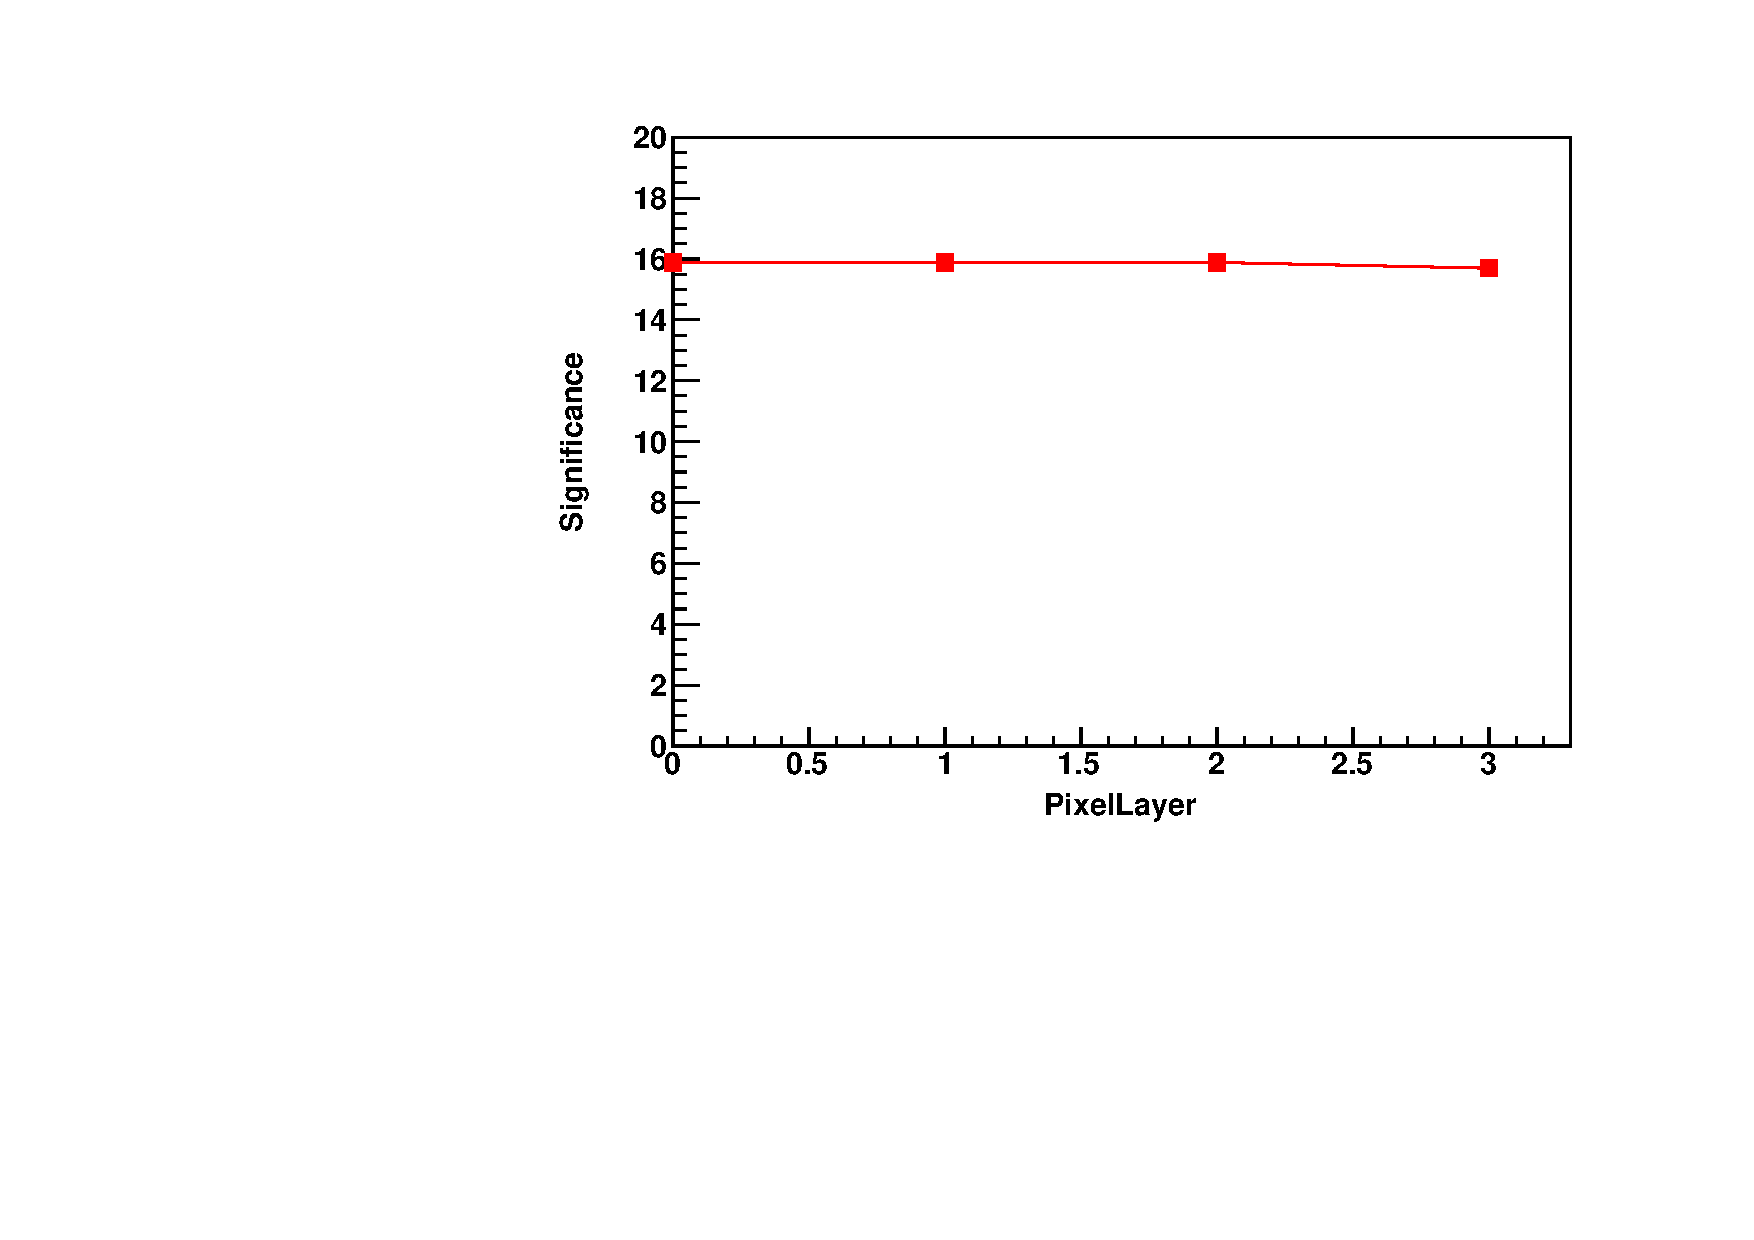
\includegraphics[angle=0,width=0.45\textwidth]{chap_YInPbPbColl2011_figures/PixelLayer_Significance1} 
   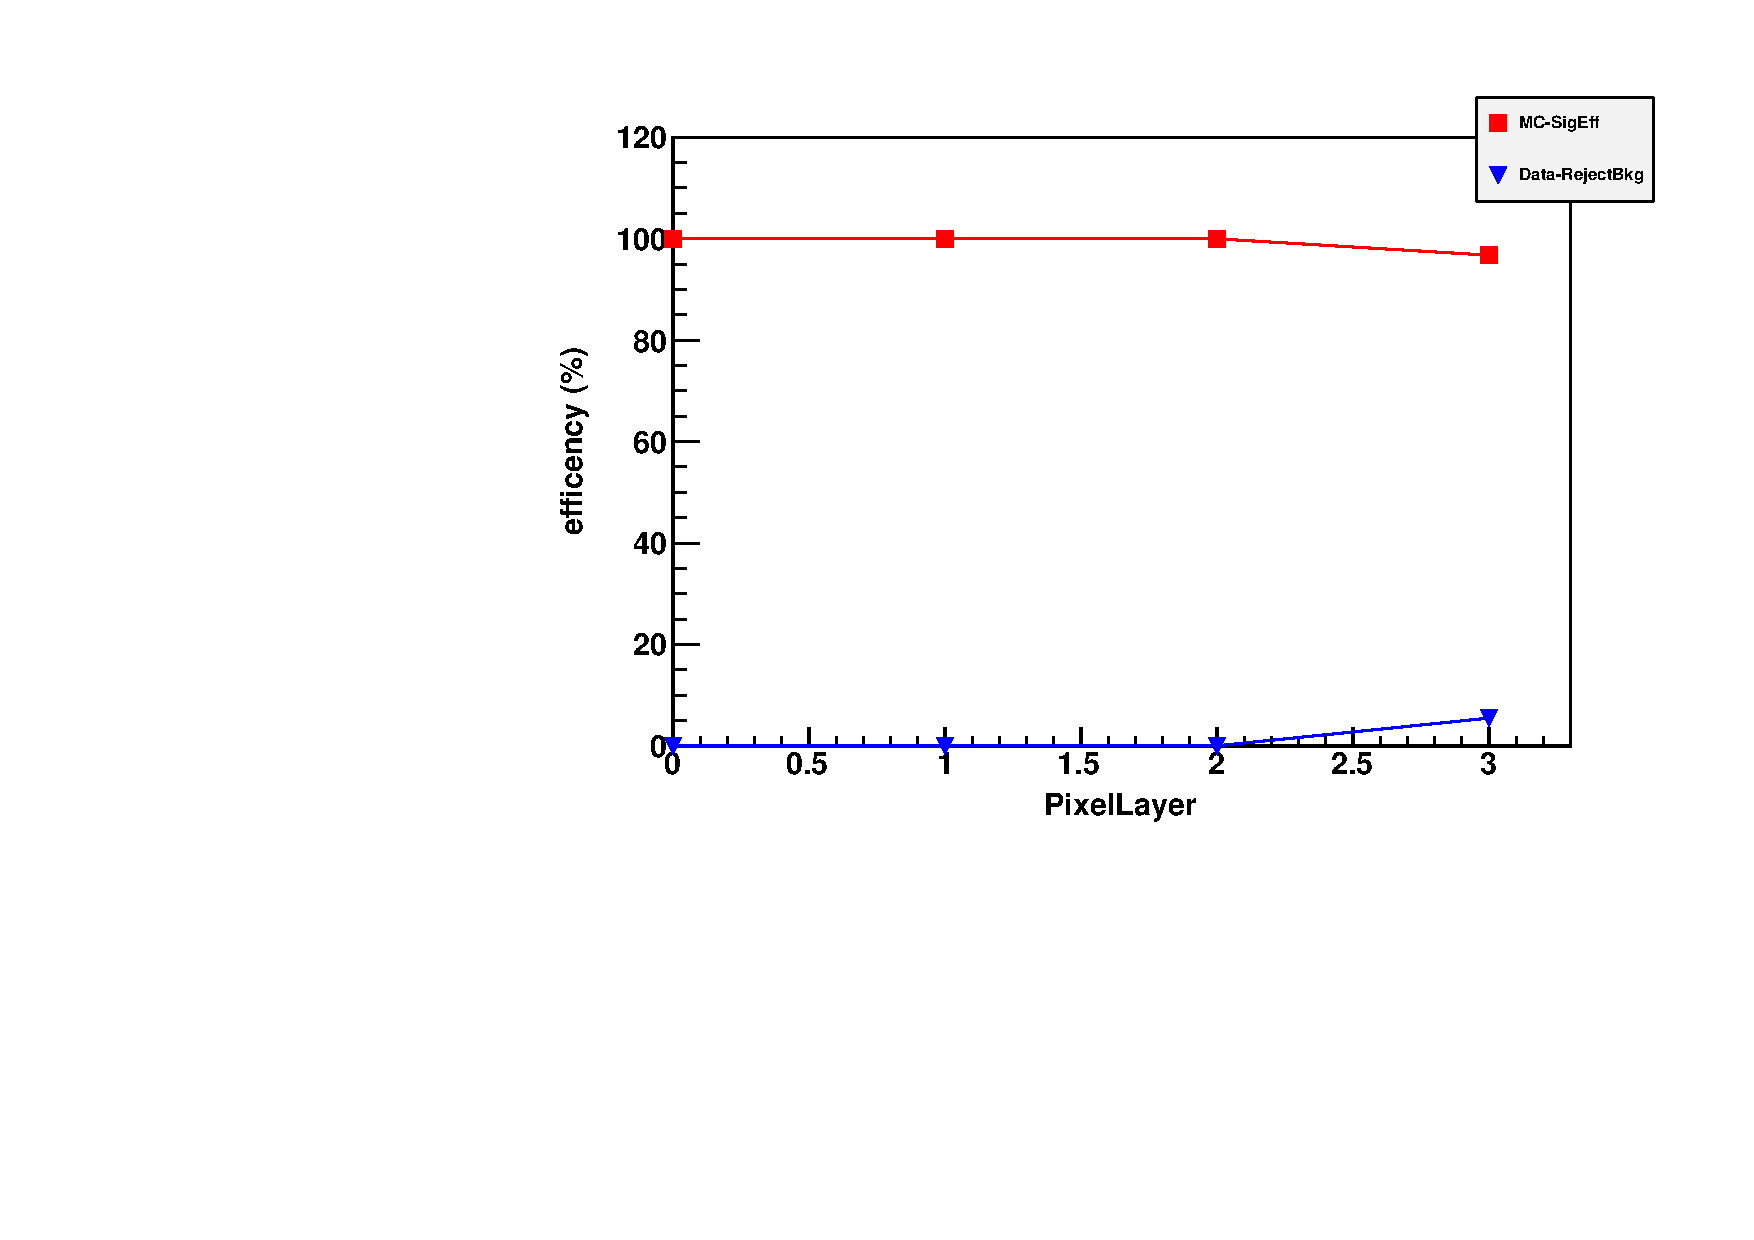
\includegraphics[angle=0,width=0.45\textwidth]{chap_YInPbPbColl2011_figures/PixelLayer_SigBkgRejEff}
   \caption{Number of muon pixel layers cut study(default: $>0$).} 
   \label{fig:mu_pixelLayers}
\end{center}
\end{figure}



Figure~\ref{fig:mu_innerTrack_chi2NDOF} shows that for the inner track $\chi^2/ndf$, the significance is mostly flat while the efficiency increases 
until about 2 and then stay maximal. The conservative cut picked is: \\ mu\_innerTrack\_chi2NDOF$<$4.
%
\begin{figure}[h!]
 \begin{center}
   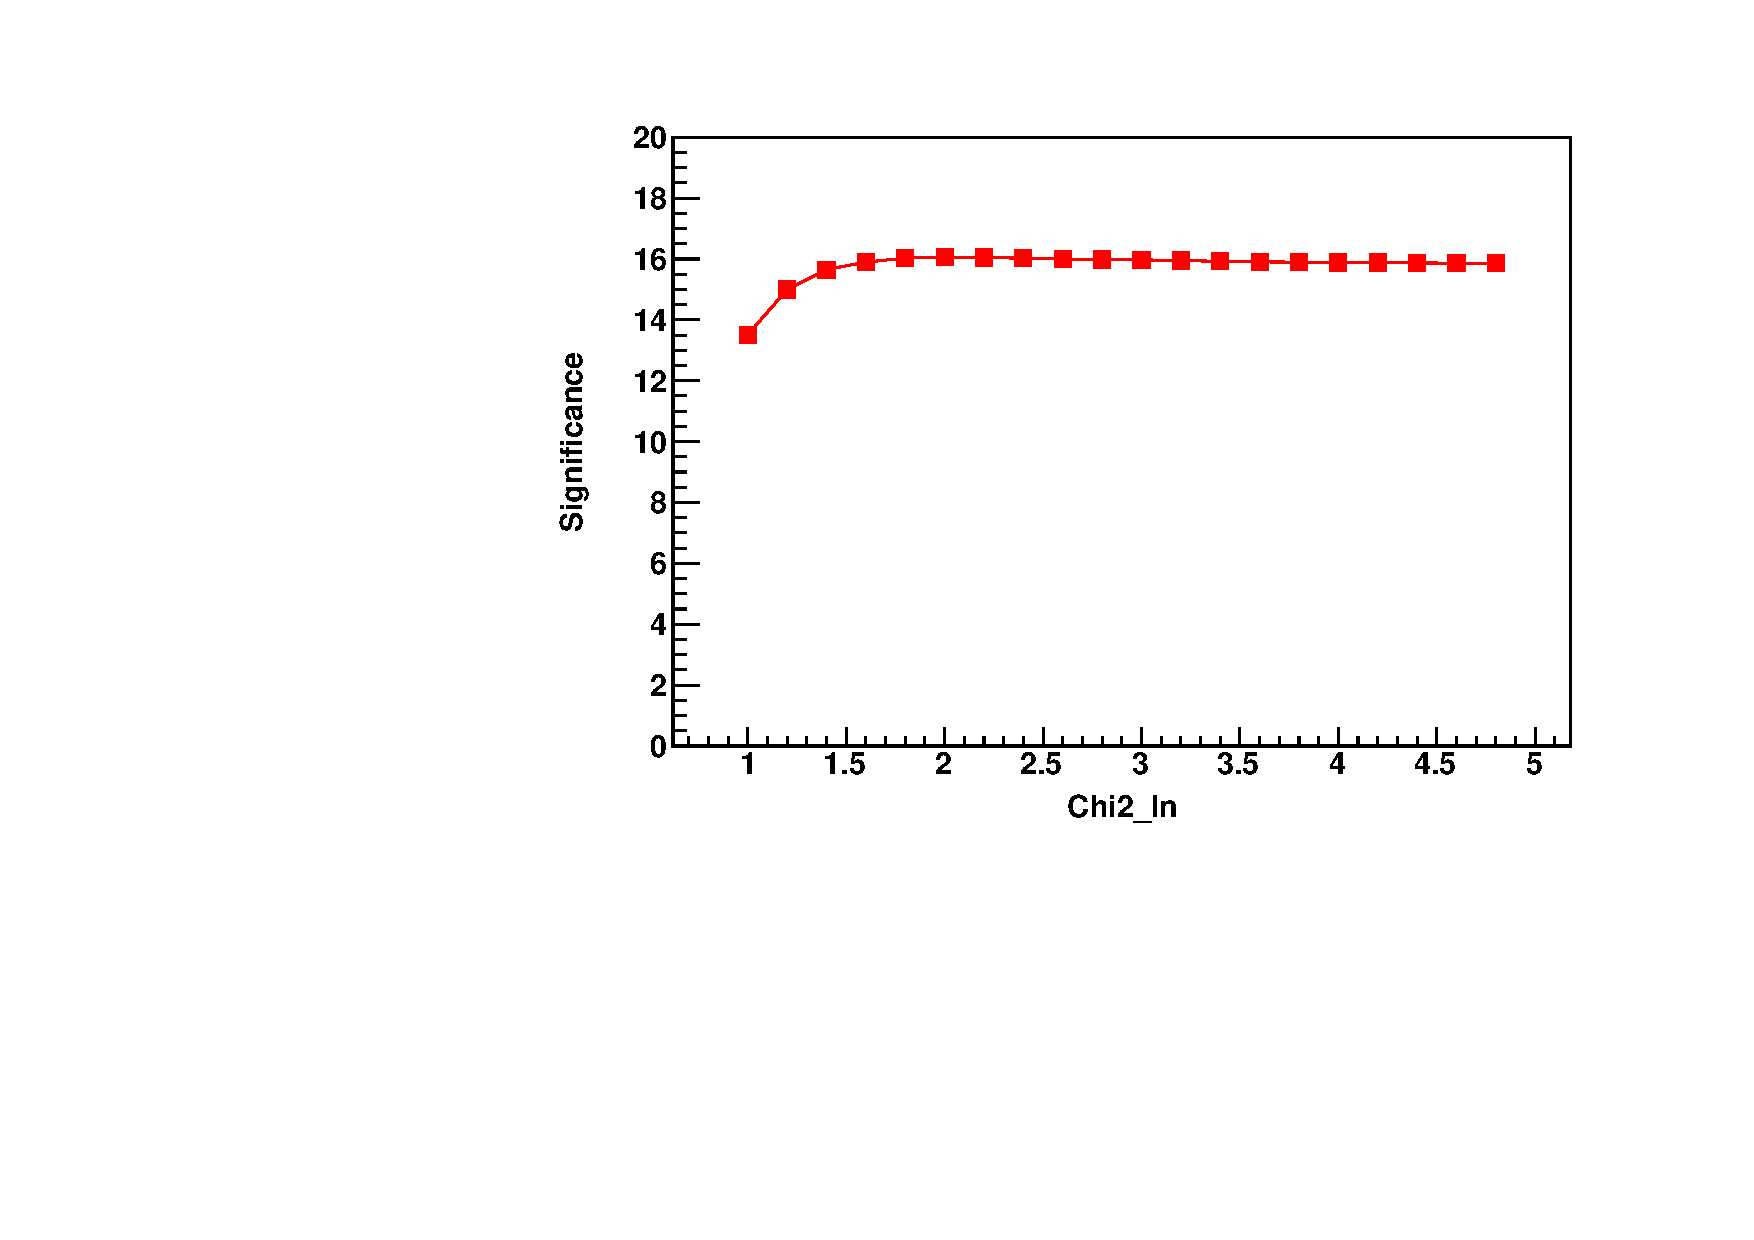
\includegraphics[angle=0,width=0.45\textwidth]{chap_YInPbPbColl2011_figures/InChi2_Significance1} 
   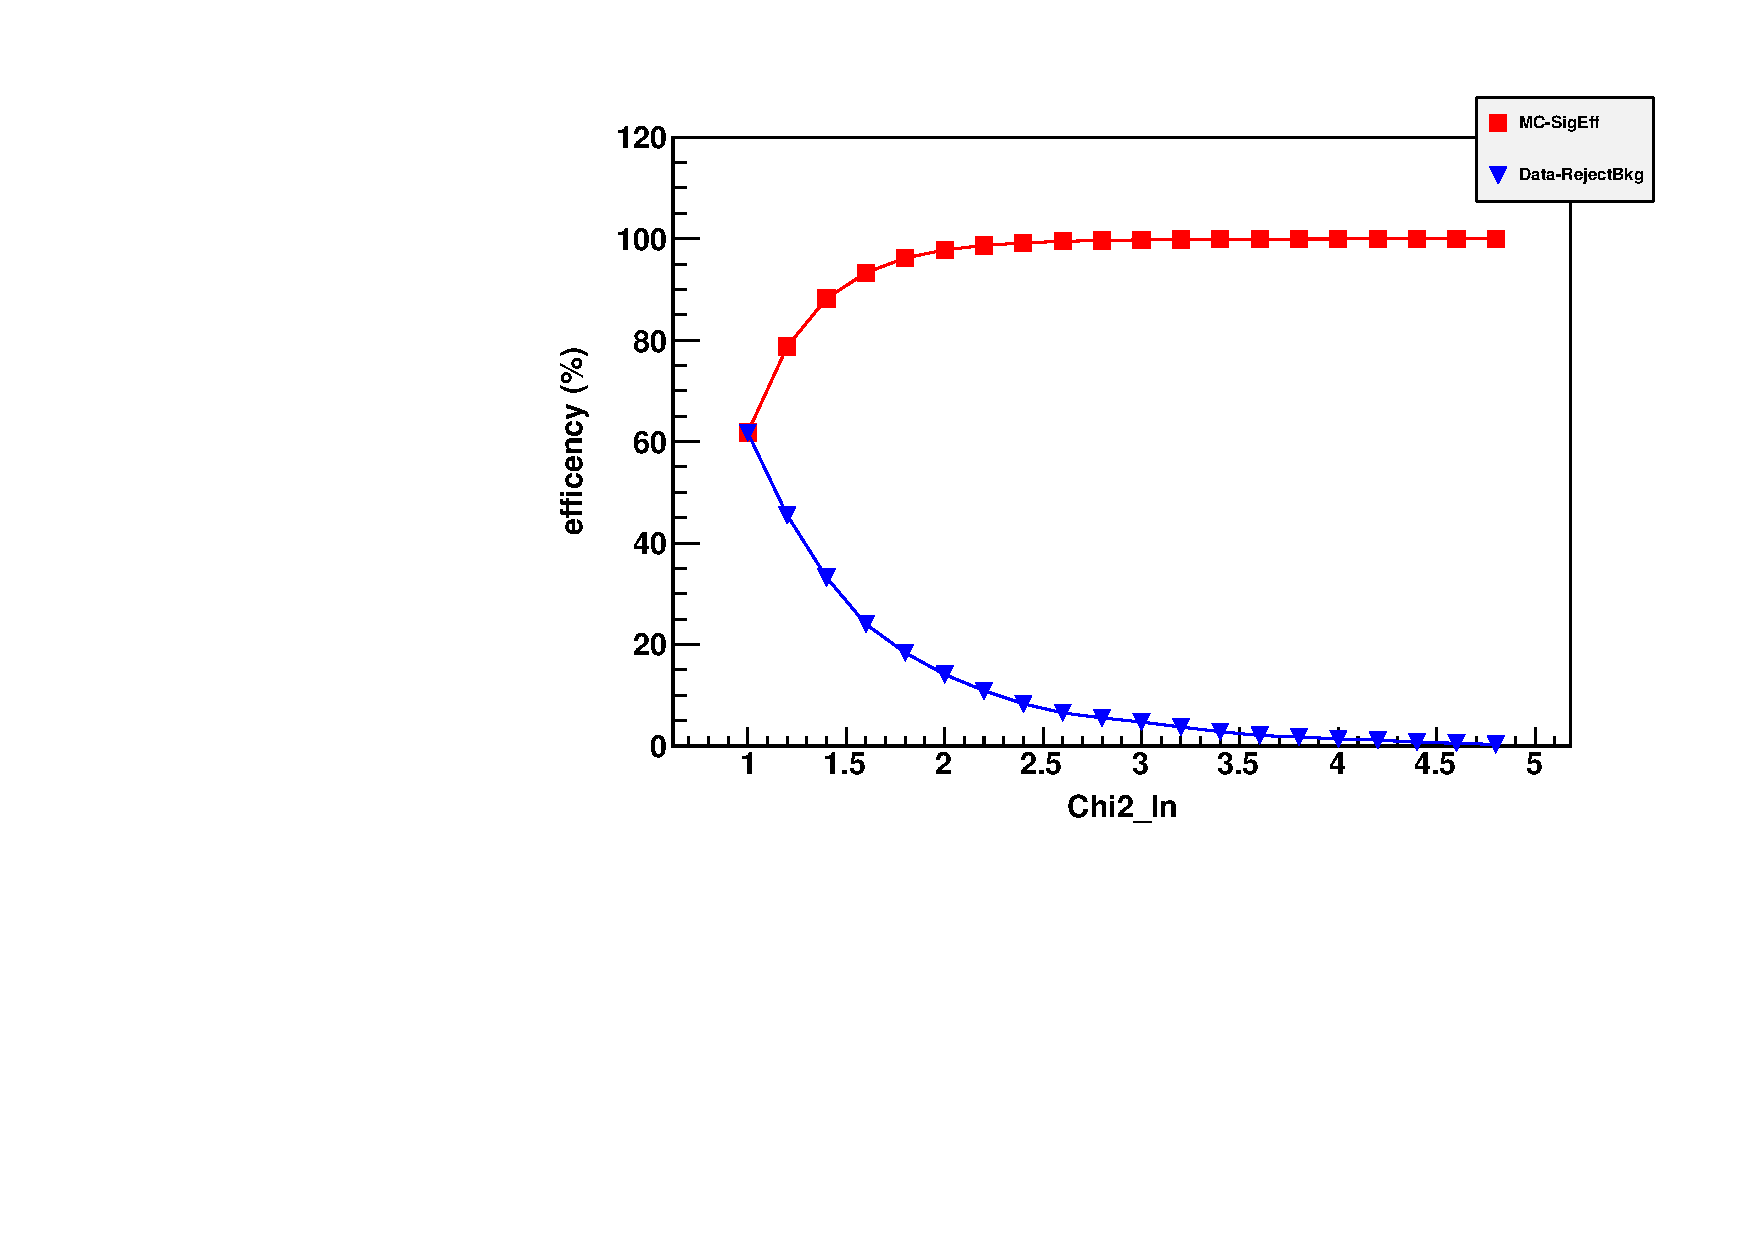
\includegraphics[angle=0,width=0.45\textwidth]{chap_YInPbPbColl2011_figures/InChi2_SigBkgRejEff}
   \caption{Number of muon inner track $\chi^2/\text{ndf}$ cut study  (default: $<4$).} %(default {\tt mu\_innerTrack\_chi2NDOF<4}).}
   %\caption{Single muon inner track  studied while applying all other cuts: left, significance on the data and right, efficiency and background rejection on MC. Final cut $<$4.}
   \label{fig:mu_innerTrack_chi2NDOF}
 \end{center}
\end{figure}

Figure~\ref{fig:mu_globalTrack_chi2NDOF} shows that for the global track $\chi^2/ndf$, the significance increases 
up to above 4 and then is constant. The conservative cut picked is: mu\_globalTrack\_chi2NDOF$<$20.
%
\begin{figure}[h!]
 \begin{center}
   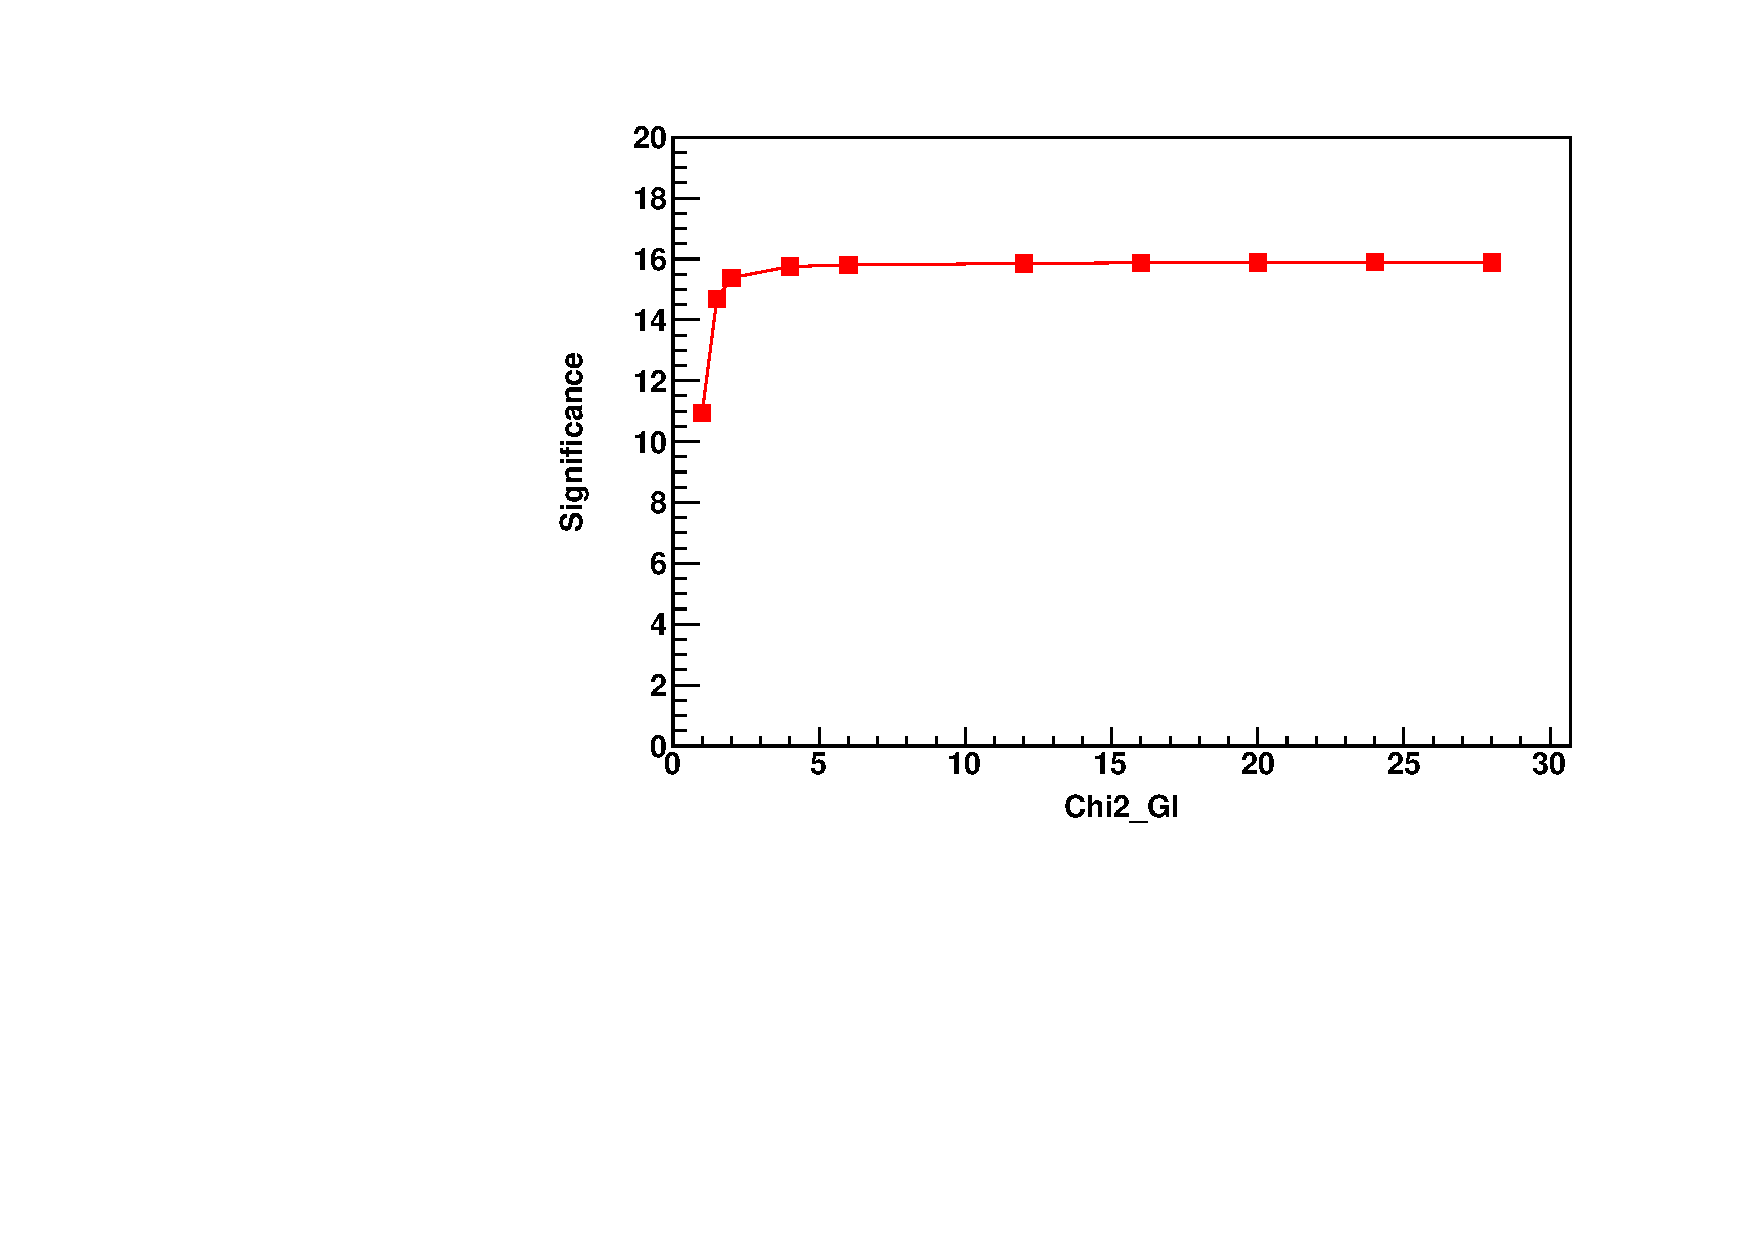
\includegraphics[angle=0,width=0.45\textwidth]{chap_YInPbPbColl2011_figures/GlChi2_Significance1}
   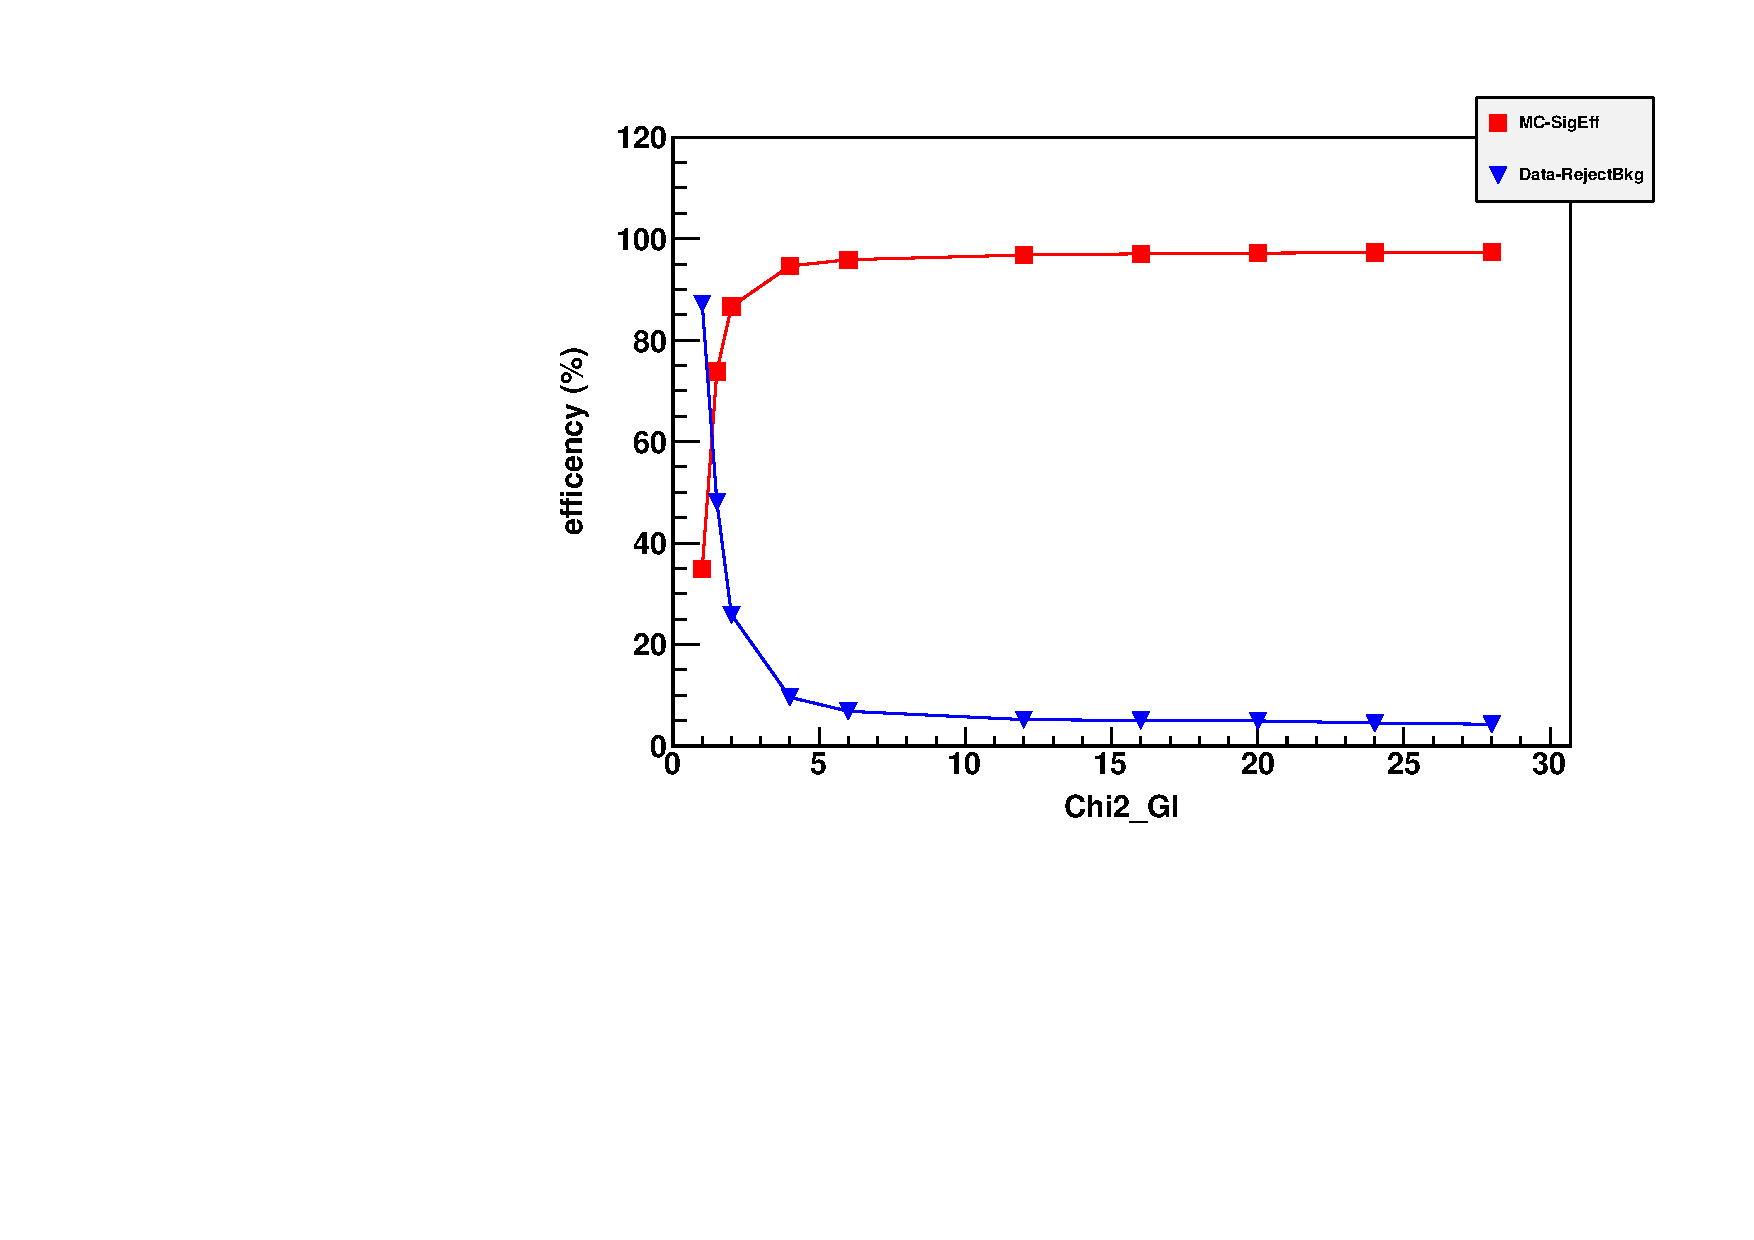
\includegraphics[angle=0,width=0.45\textwidth]{chap_YInPbPbColl2011_figures/GlChi2_SigBkgRejEff}
   \caption{Number of muon global track $\chi^2/\text{ndf}$ cut study  (default: $<20$).} %(default {\tt mu\_globalTrack\_chi2NDOF<20).}}
   %\caption{Single muon global track $\chi^2/ndf$ studied while applying all other cuts: left, significance on the data and right, efficiency and background rejection on MC. Final cut $<$20.}
   \label{fig:mu_globalTrack_chi2NDOF}
 \end{center}
\end{figure}


\begin{figure}[h!]
 \begin{center}
   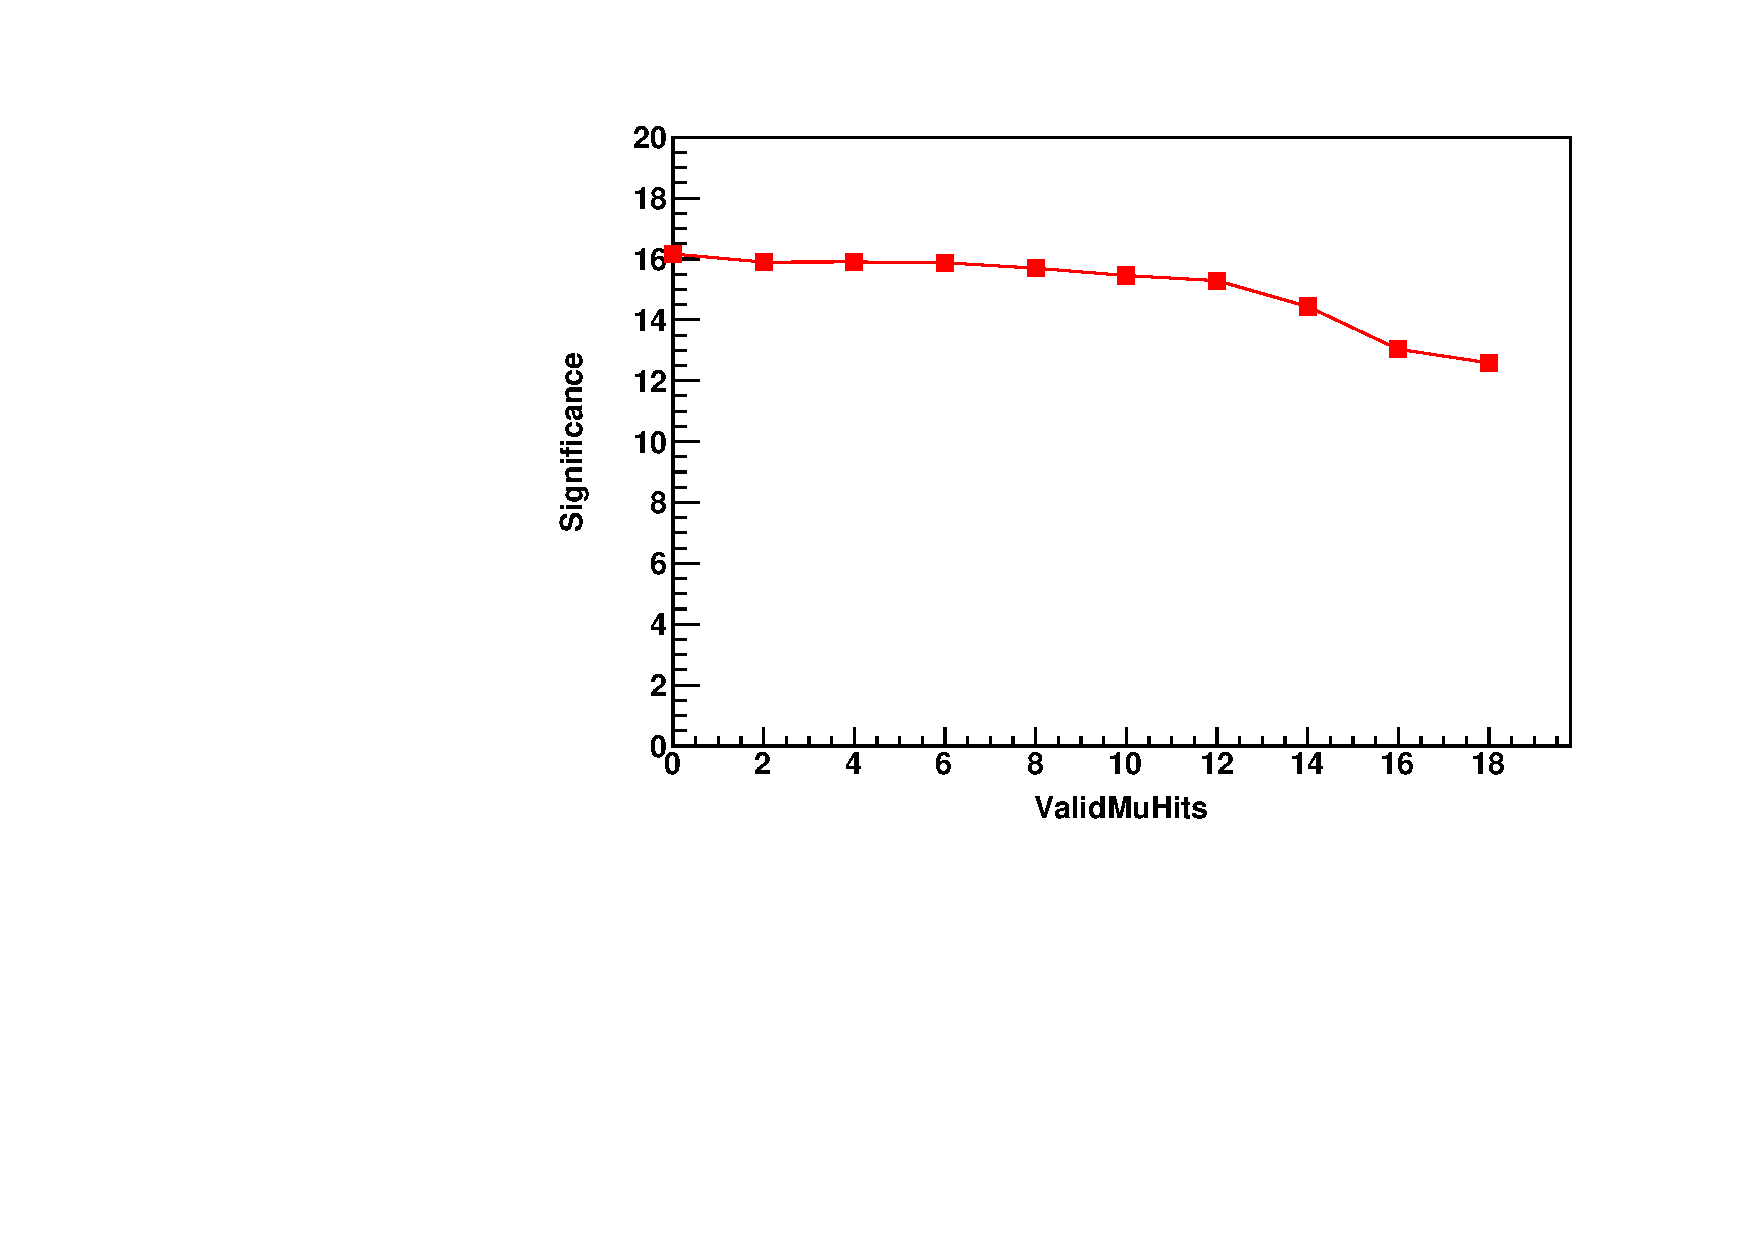
\includegraphics[angle=0,width=0.45\textwidth]{chap_YInPbPbColl2011_figures/ValidMuHits_Significance1}
   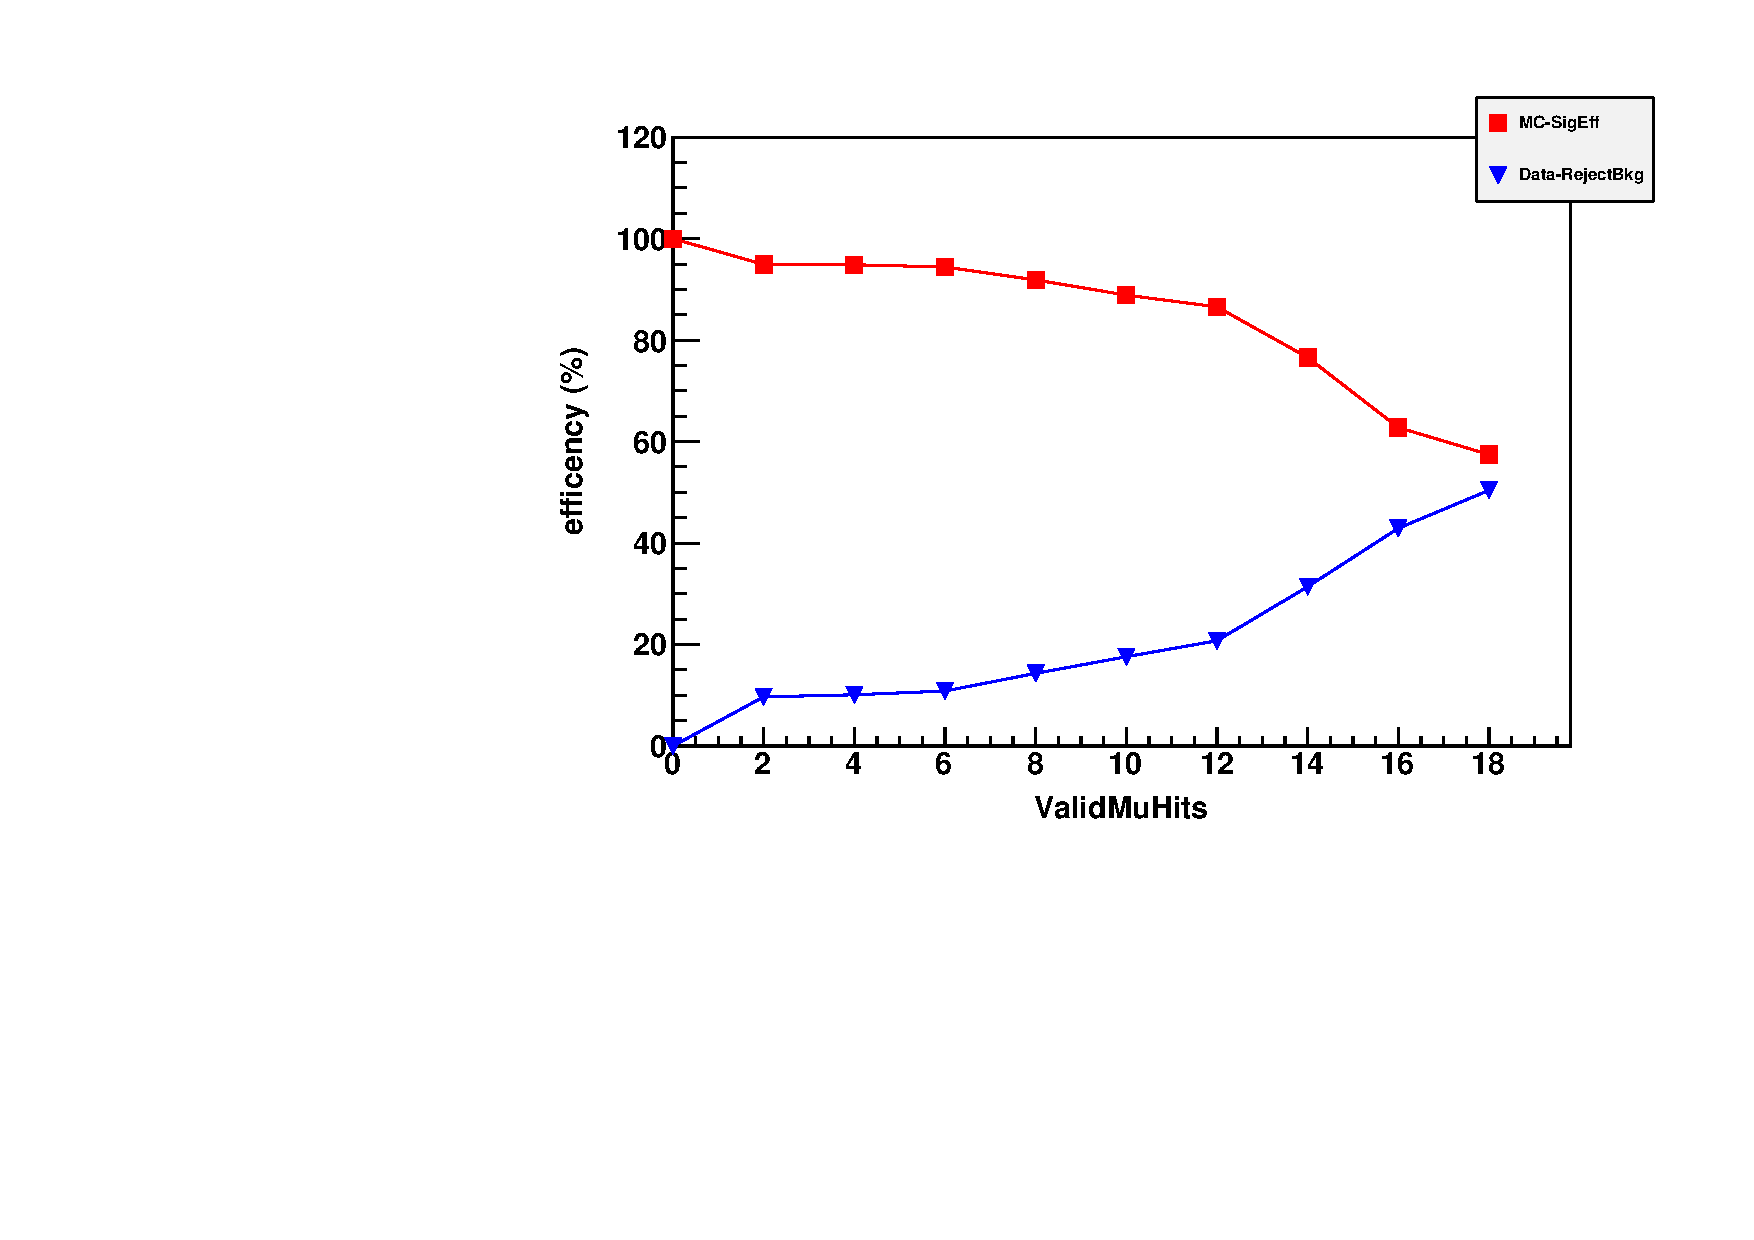
\includegraphics[angle=0,width=0.45\textwidth]{chap_YInPbPbColl2011_figures/ValidMuHits_SigBkgRejEff}
   \caption{Number of valid muon hits cut study  (default: $\geq 0$).} %(default {\tt mu\_globalTrack\_chi2NDOF<20).}}
   %\caption{Single muon global track $\chi^2/ndf$ studied while applying all other cuts: left, significance on the data and right, efficiency and background rejection on MC. Final cut $<$20.}
   \label{fig:muun_valid_hits}
 \end{center}
\end{figure}

Figures~\ref{fig:mu_Dxy} and ~\ref{fig:mu_Dz} shows the significance on data and the efficiency and background rejection 
on MC for different values of $D_{xy}$ and $D_z$ while applying all other cuts. The final cuts are chosen:
 mu\_dxy$<$3.0~cm and mu\_dz$<$15.0~cm.
%
\begin{figure}[h!]
 \begin{center}
   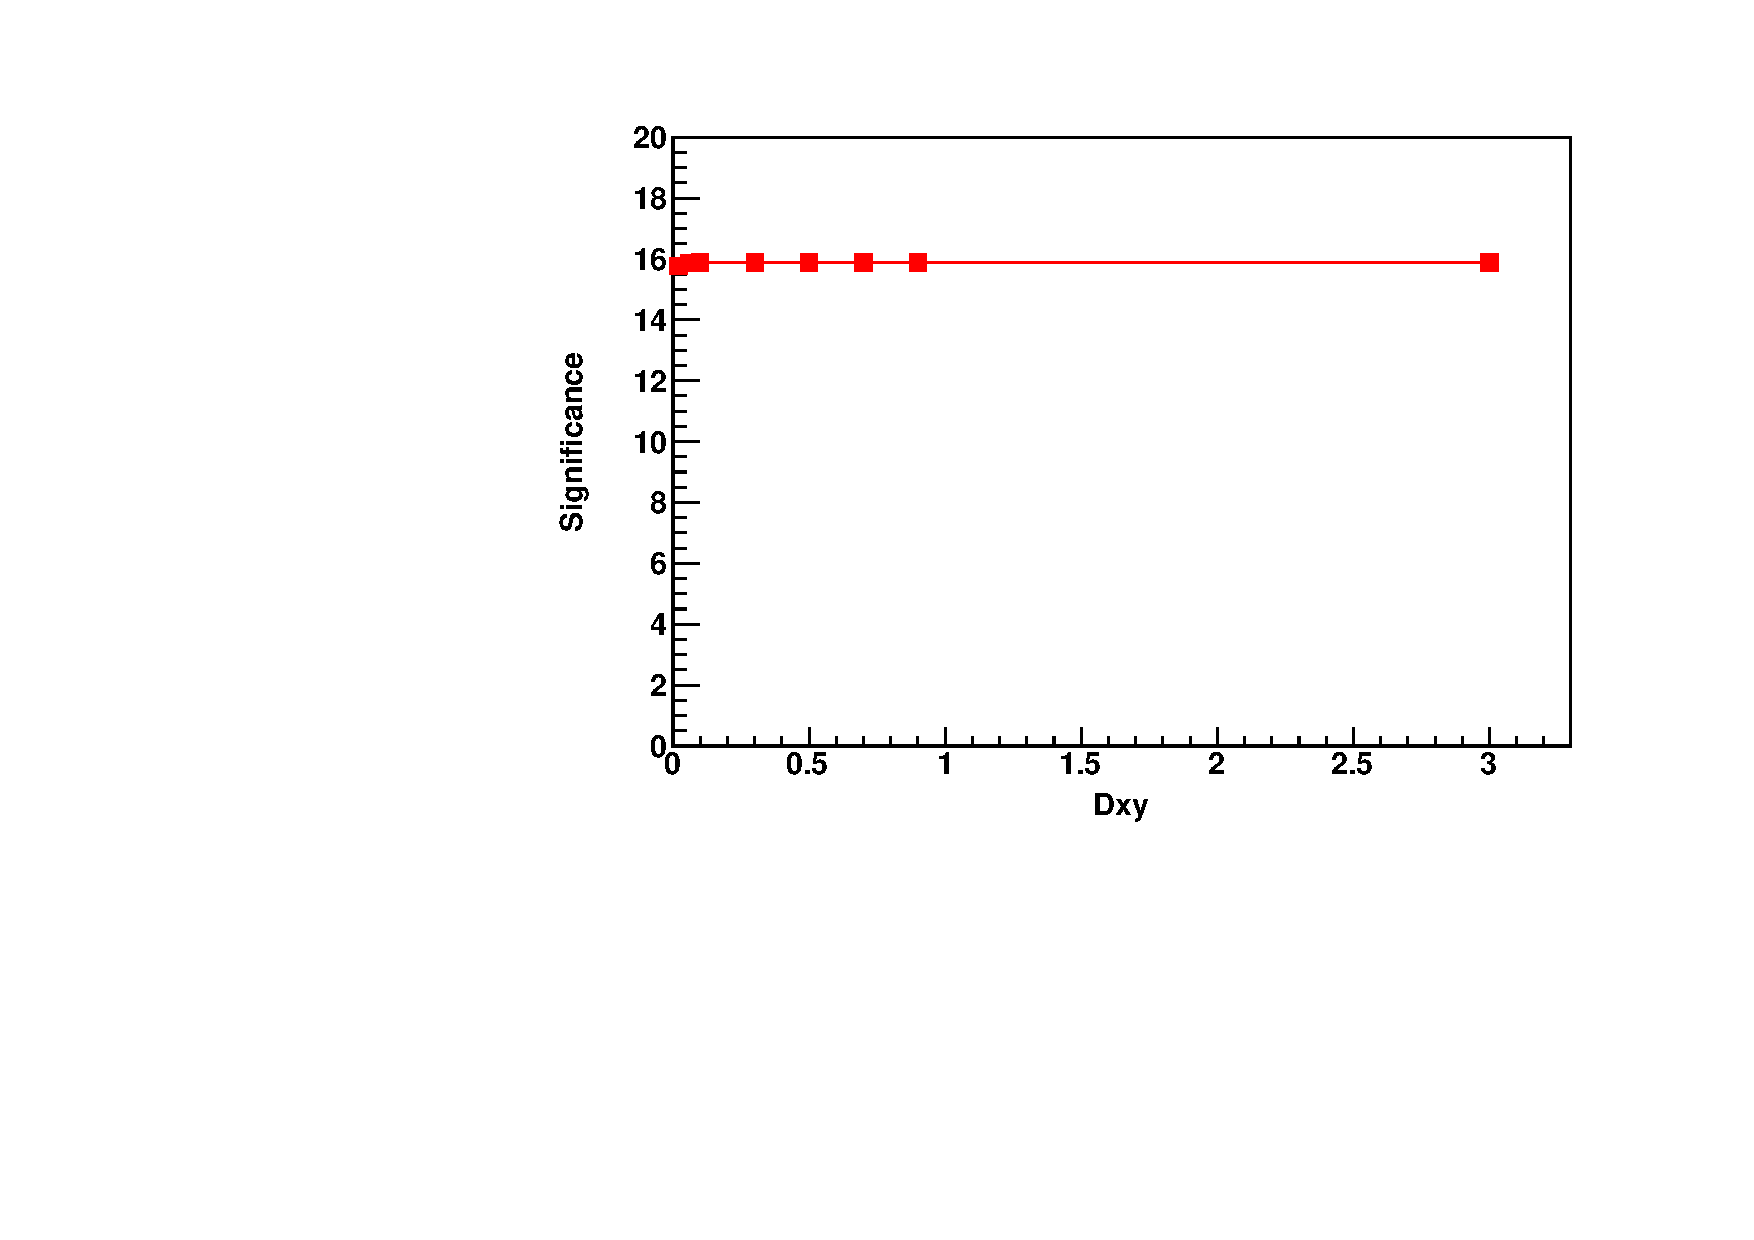
\includegraphics[angle=0,width=0.45\textwidth]{chap_YInPbPbColl2011_figures/Dxy_Significance1} 
   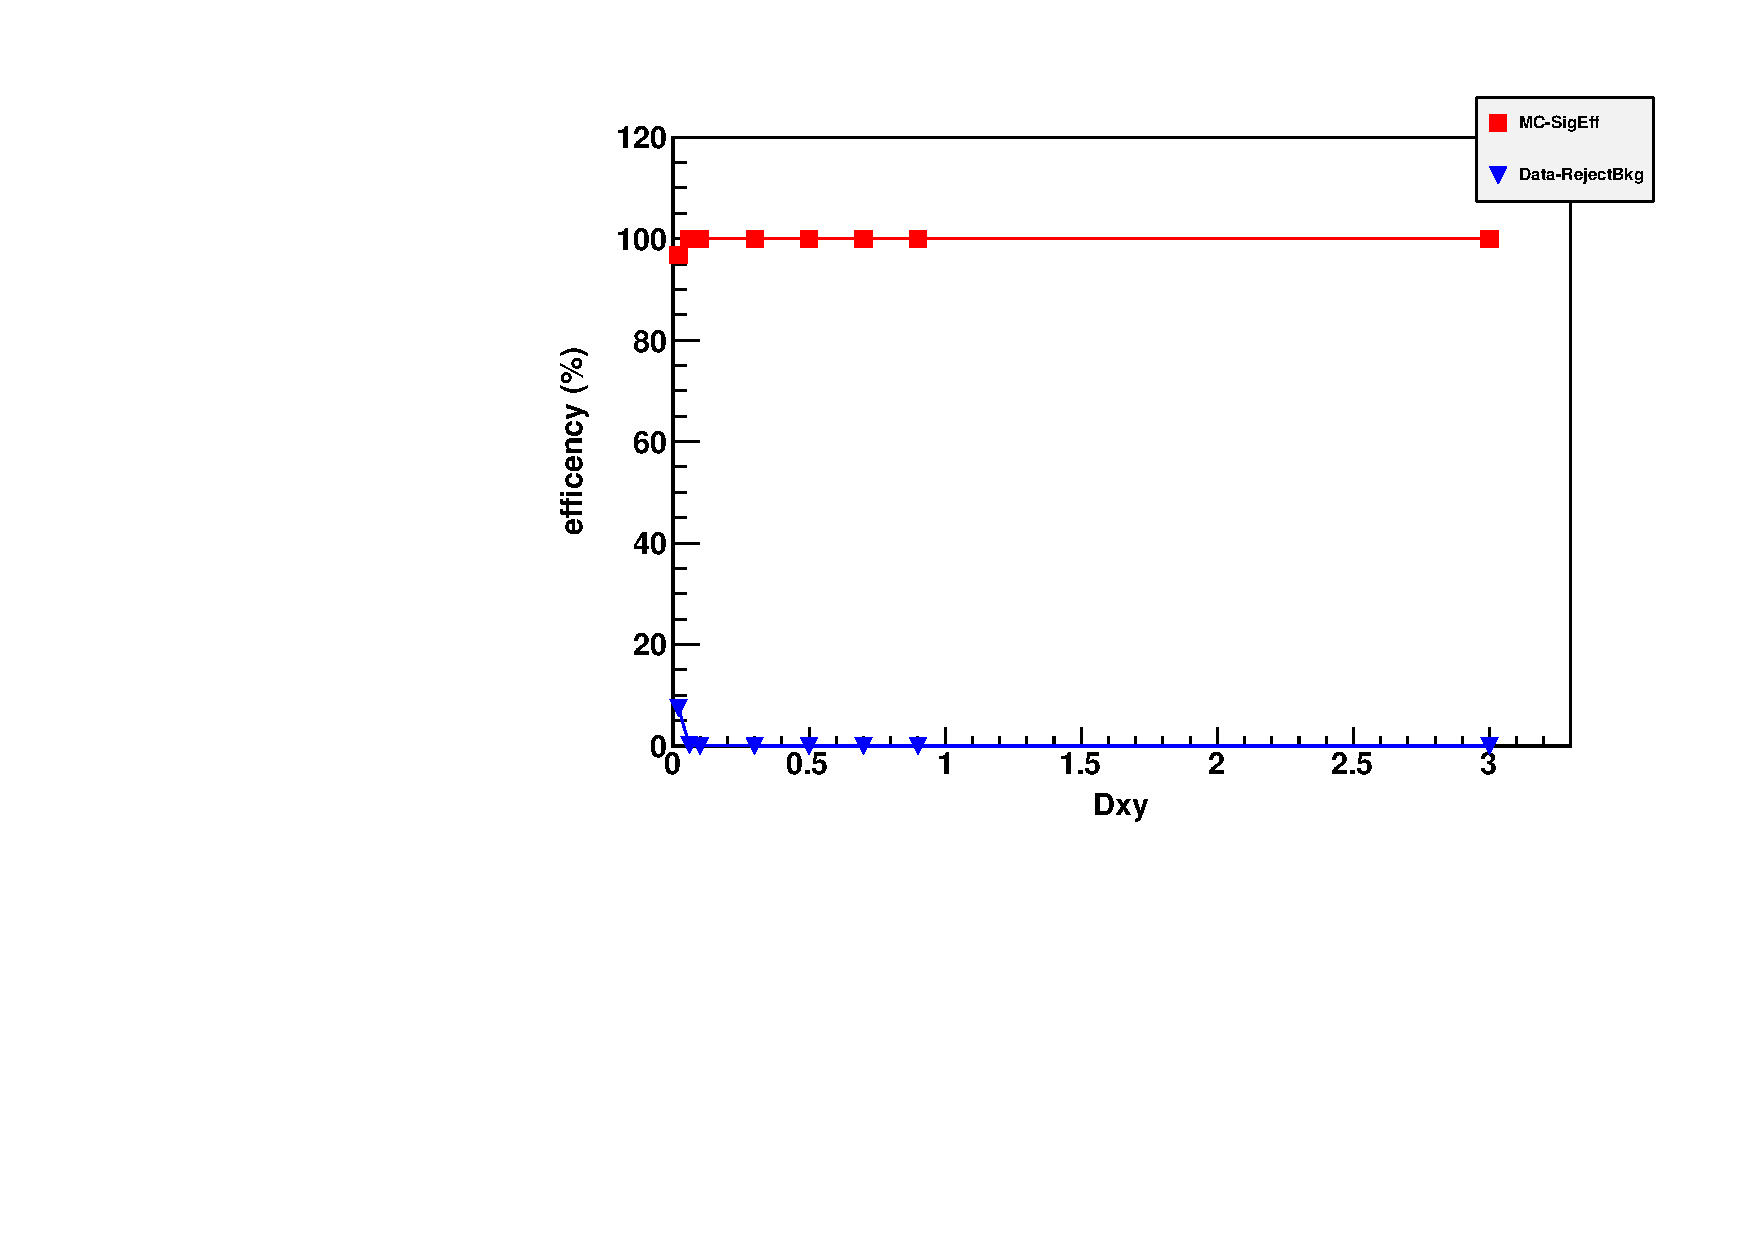
\includegraphics[angle=0,width=0.45\textwidth]{chap_YInPbPbColl2011_figures/Dxy_SigBkgRejEff}
   \caption{$D_{xy}$ cut study  (default: $<3$).} %(default {\tt $D_{xy}<3$).}} 
   %\caption{$D_{xy}$ study while applying all other cuts: left, significance on the data and right, efficiency and background rejection on MC.}
   \label{fig:mu_Dxy}
 \end{center}
\end{figure}
%
\begin{figure}[h!]
 \begin{center}
   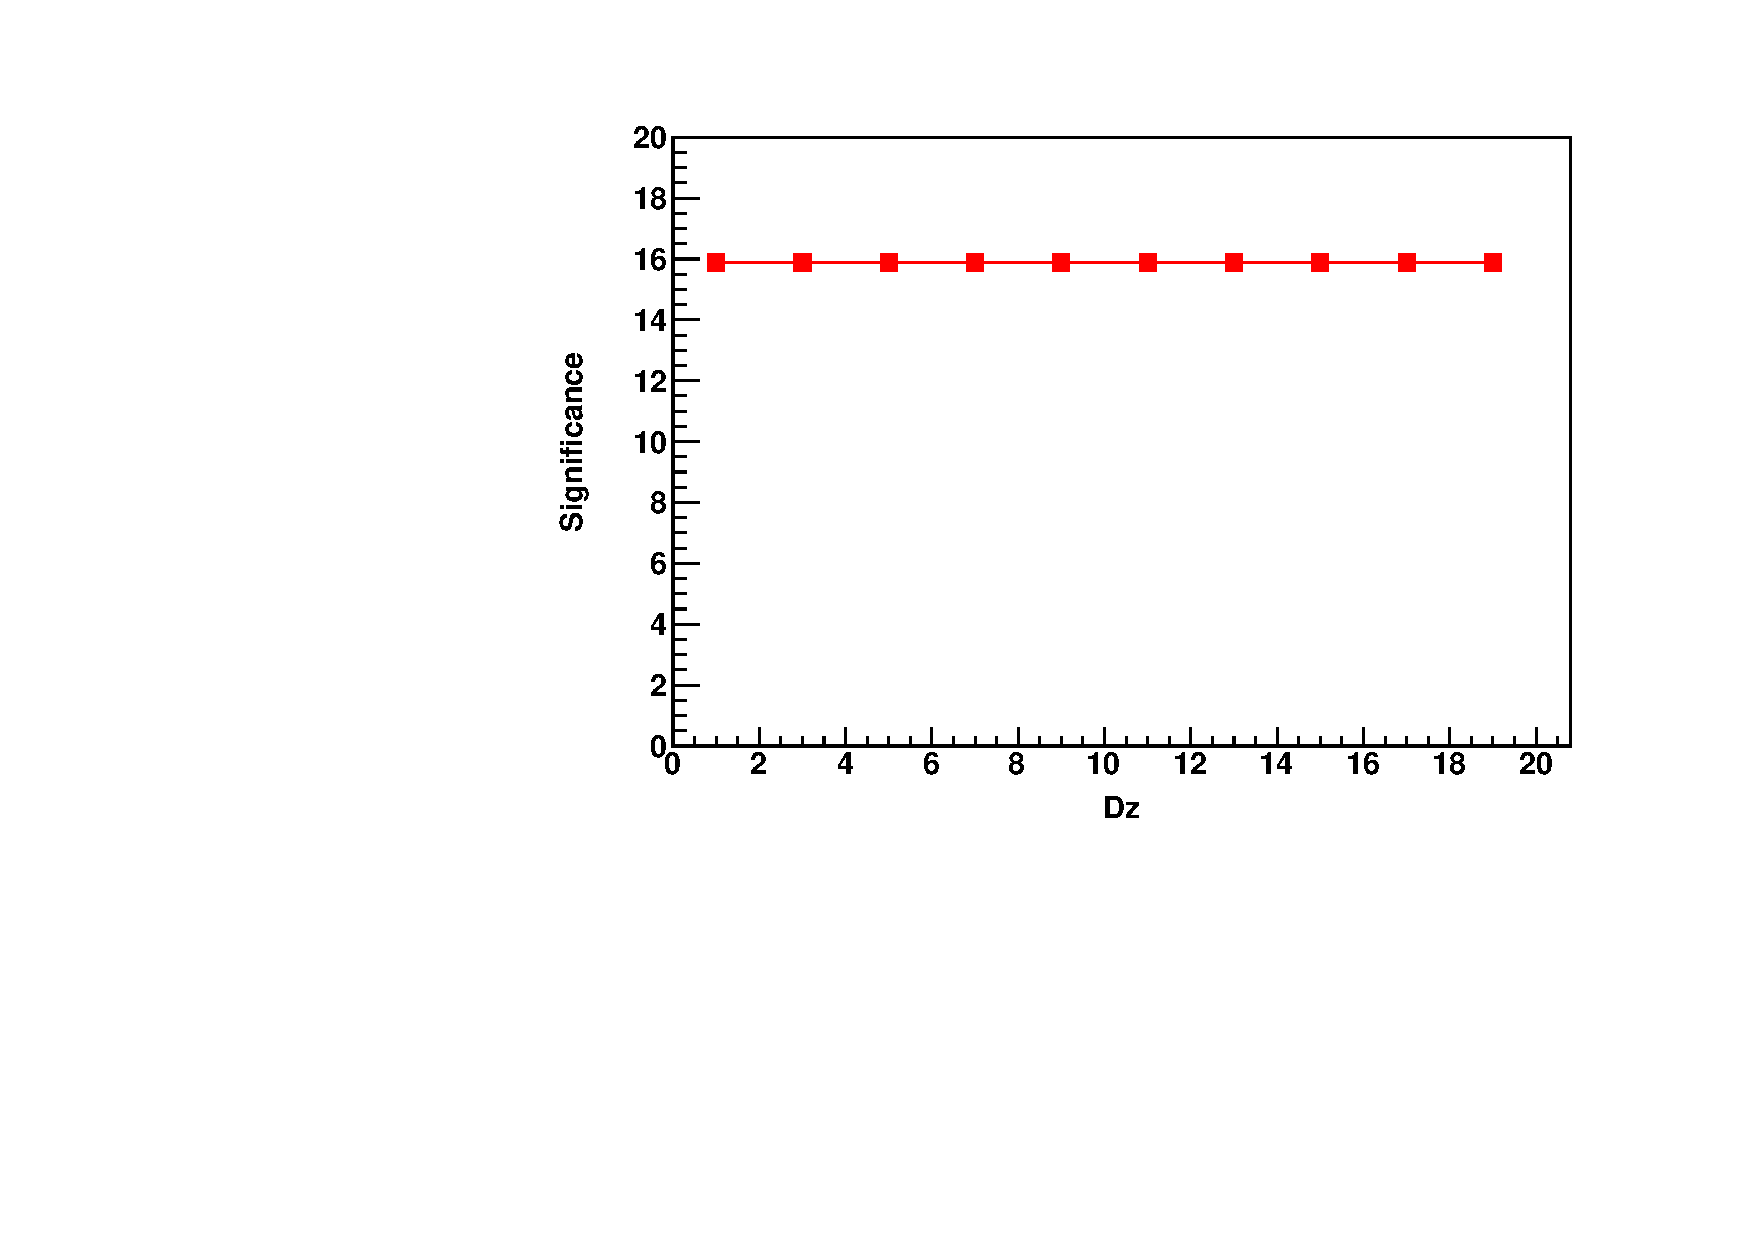
\includegraphics[angle=0,width=0.45\textwidth]{chap_YInPbPbColl2011_figures/Dz_Significance1} 
   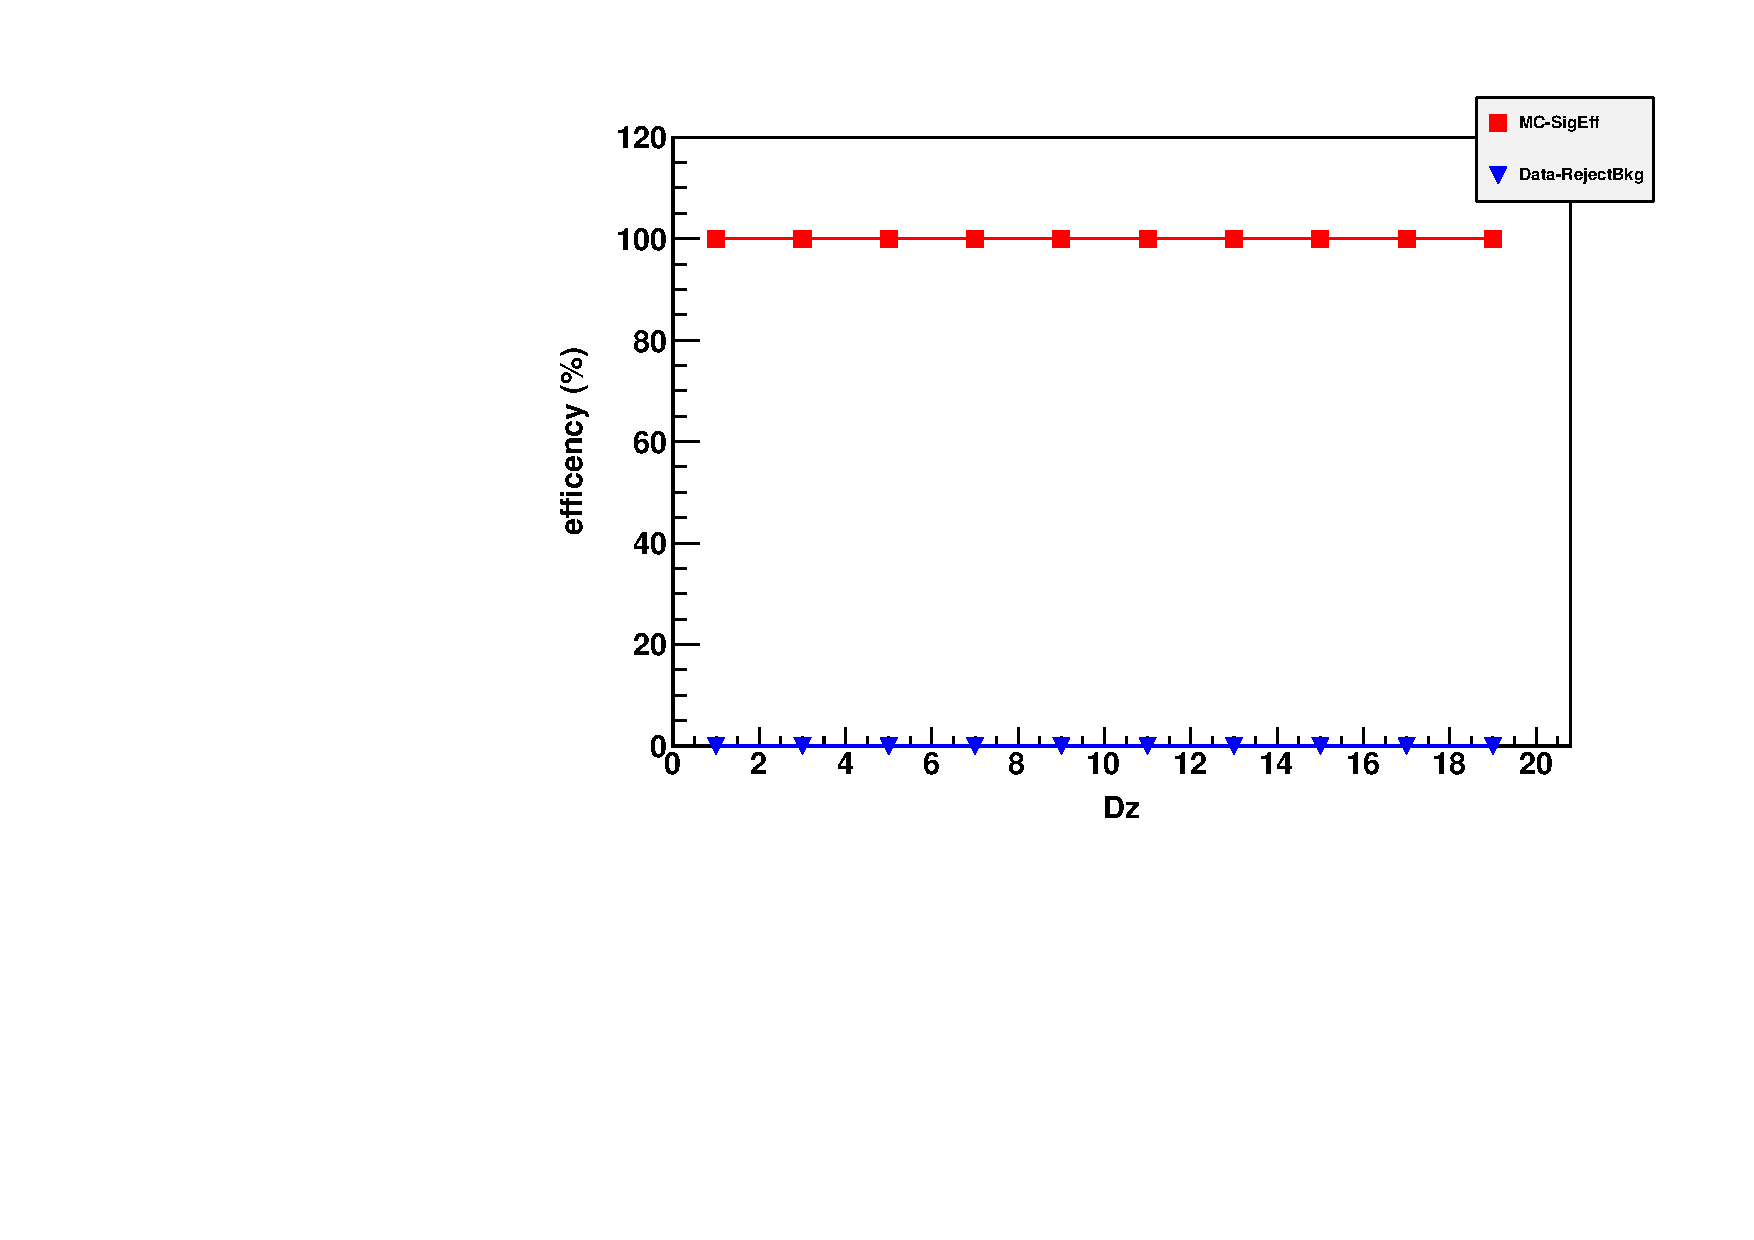
\includegraphics[angle=0,width=0.45\textwidth]{chap_YInPbPbColl2011_figures/Dz_SigBkgRejEff}
   \caption{$D_{z}$ cut study  (default: $<15$).} %(default {\tt $D_{z}<15$).}} 
   %\caption{$D_{z}$ study while applying all other cuts: left, significance on the data and right, efficiency and background rejection on MC.}
   \label{fig:mu_Dz}
 \end{center}
\end{figure}

Figures~\ref{fig:mu_vprob} show for for the vertex probability study, the significance is constant 
as all other cuts are applied. A reasonable 5\% cut for the vertex probability is chosen.
%
\begin{figure}[h!]
 \begin{center}
   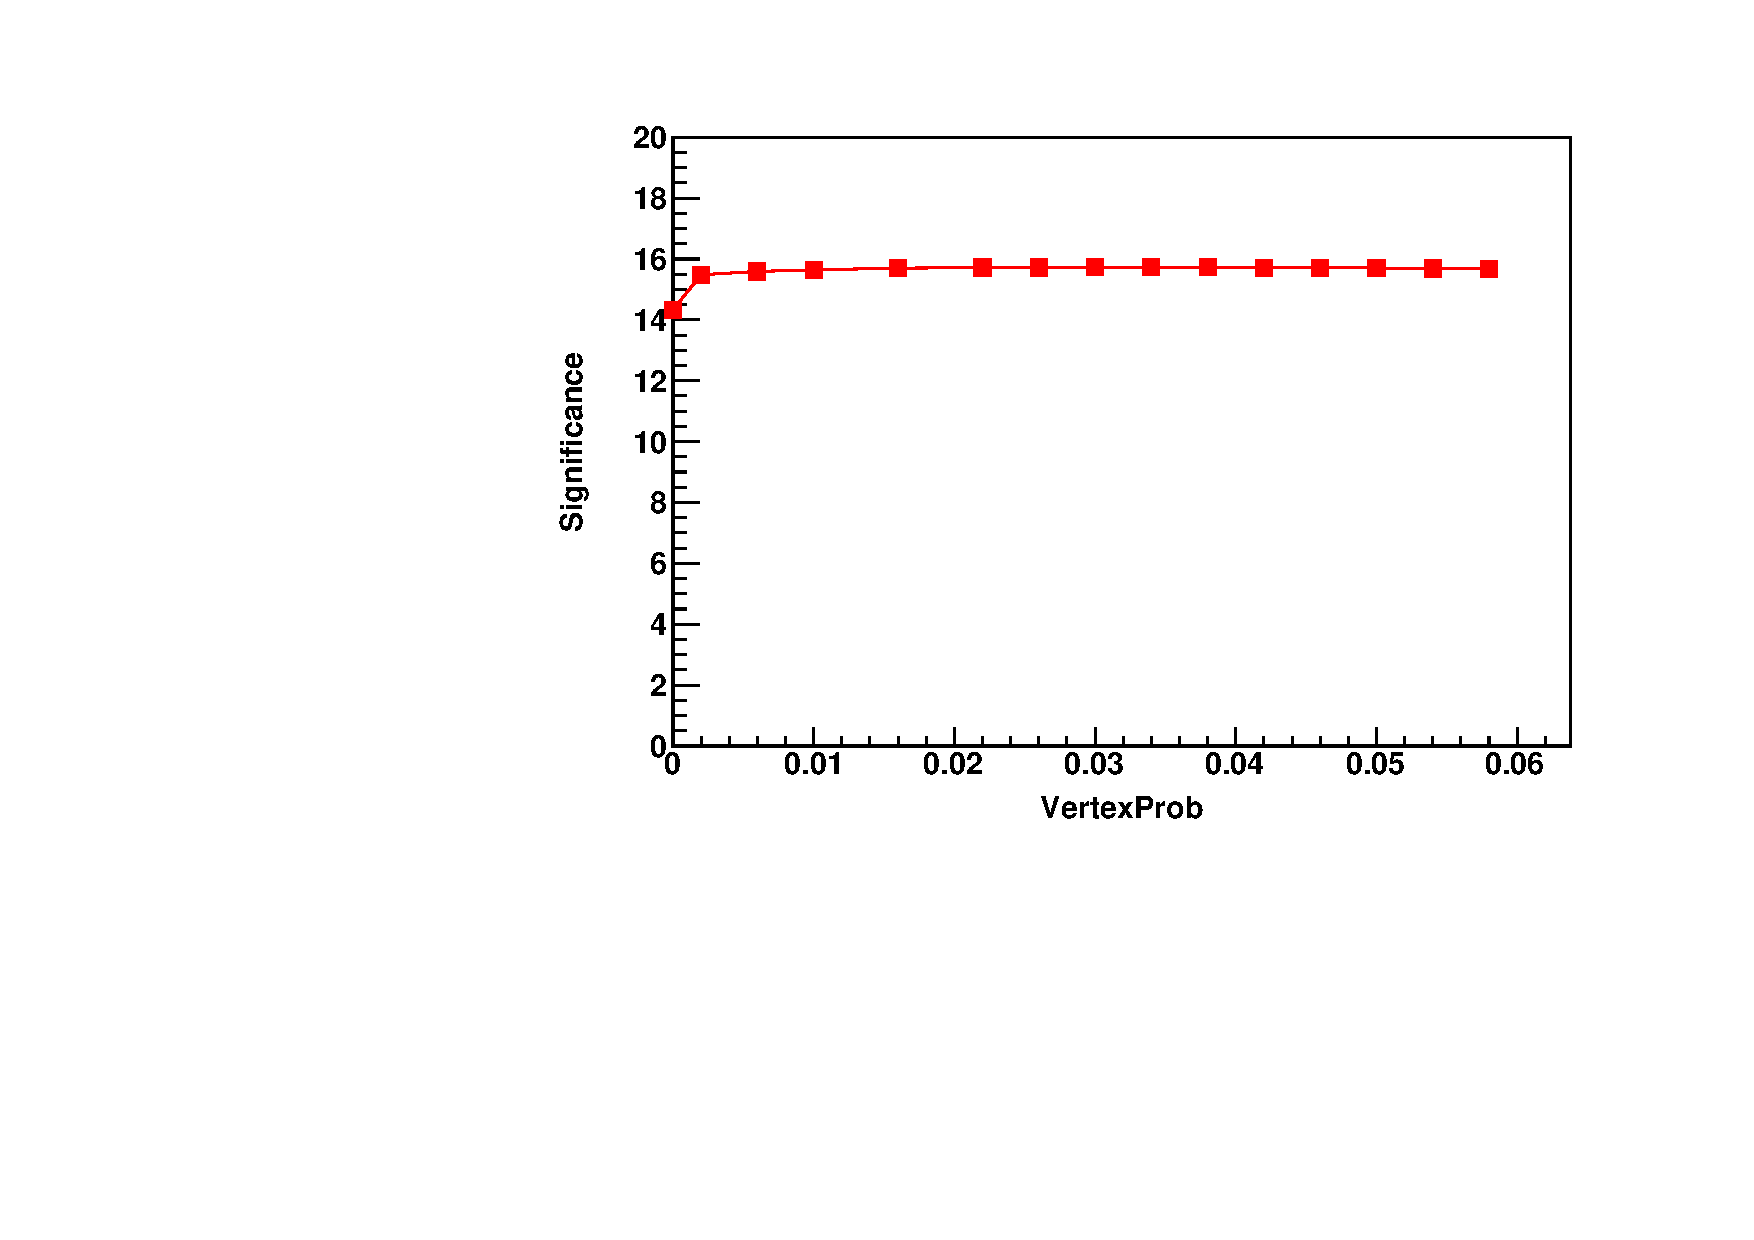
\includegraphics[angle=0,width=0.45\textwidth]{chap_YInPbPbColl2011_figures/VProb_Significance1} 
   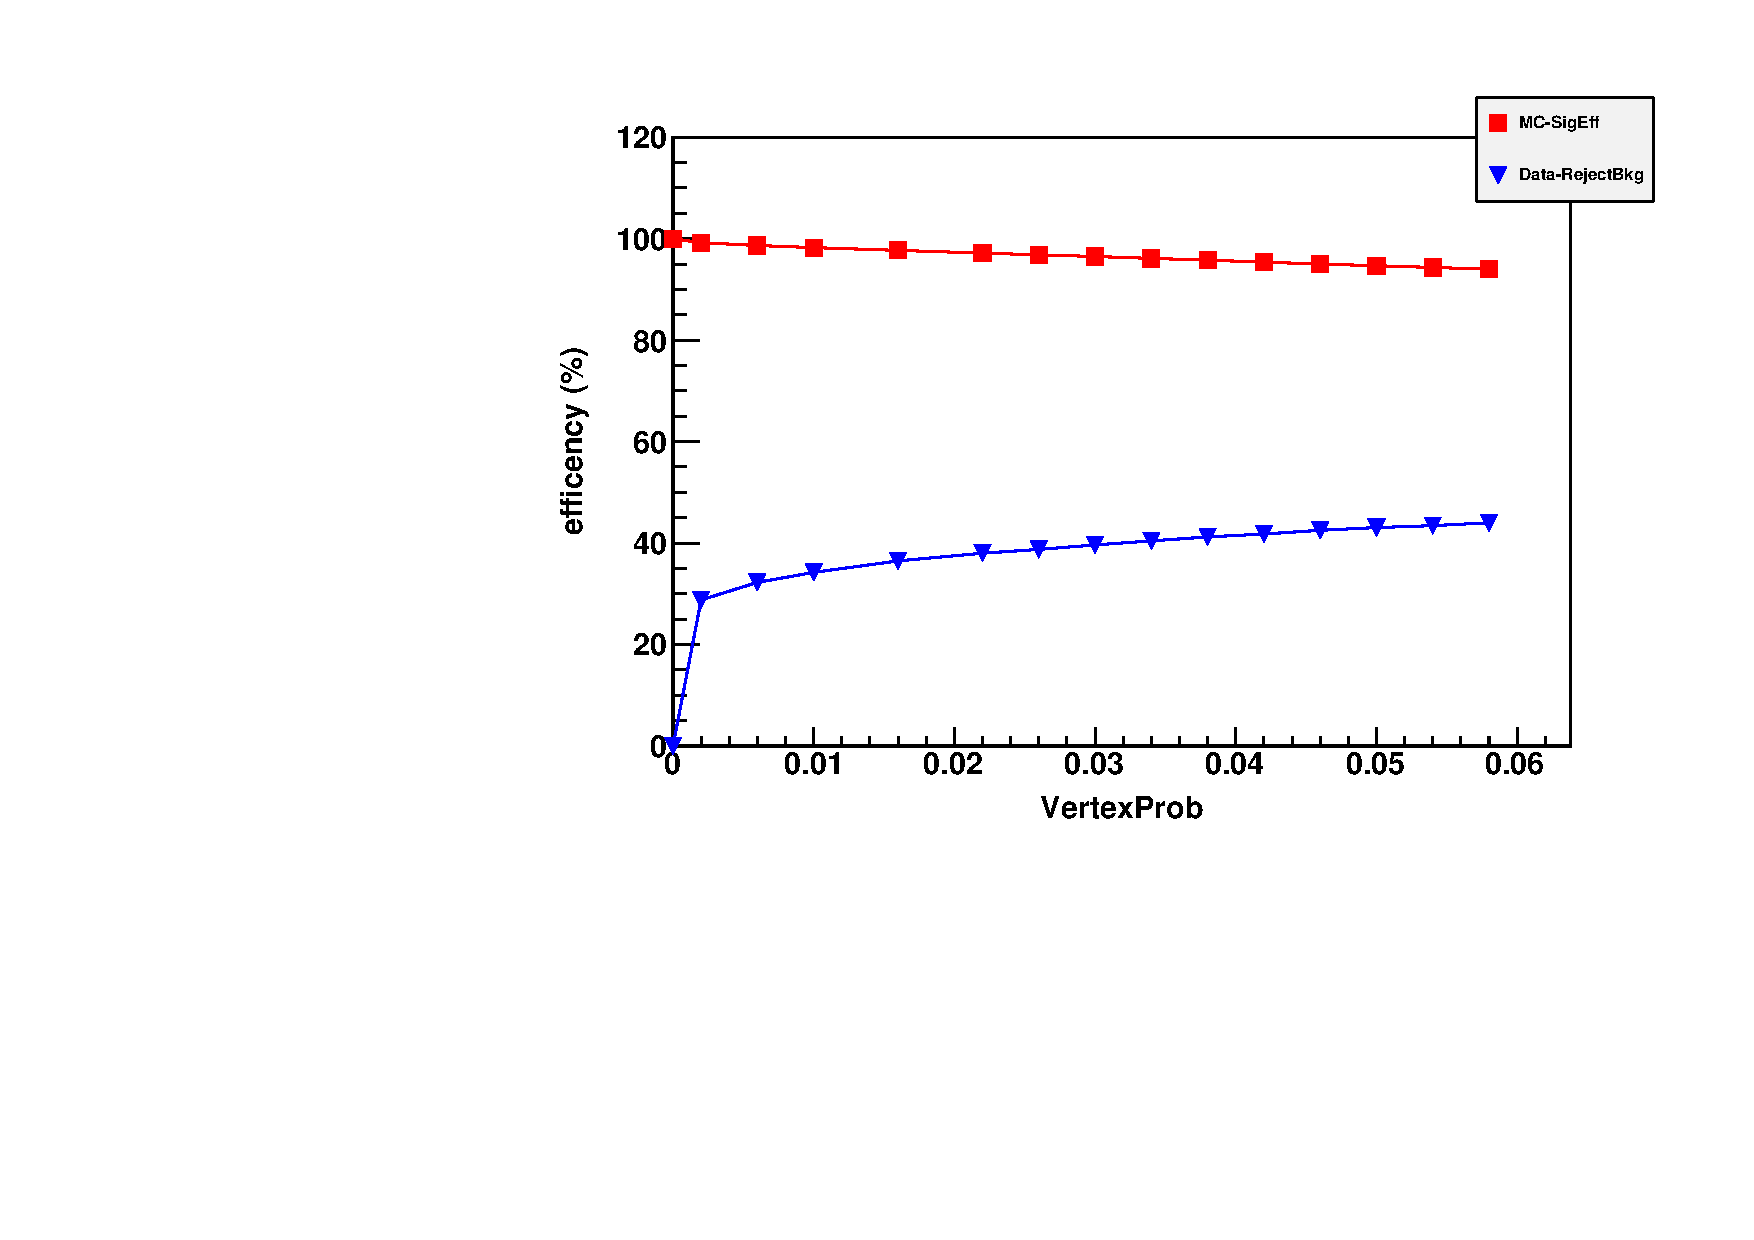
\includegraphics[angle=0,width=0.45\textwidth]{chap_YInPbPbColl2011_figures/VProb_SigBkgRejEff}
   \caption{Dimuon vertex probability cut study  (default: $>5\%$).}
   \label{fig:mu_vprob}
 \end{center}
\end{figure}

It is to be noted that the arbitration cut (the requirement of the muon to be both  
global and tracker muon) has already a very good efficiency, and thus is applied in the final set of quality criteria.


\subsection{Kinematic threshold}
\label{sec:shoulder}

The single muon $\pt$ cut was chosen according to the described optimization procedure considering also the effect of the $\pt$ cut on the shape of the background.

\subsubsection{Statistical optimization}

The optimization of the single muon $\pt$ cut is here based on the 1S peak singificance, as in Eq.~\ref{eqn:peak_signif}. Similarly to what was already described above,   
the signal is determined from MC counting the dimuons falling into the $\pm 100 \MeVcc$ mass window around the $\PgU(1S)$ peak normalized to the signal in data. 
The signal level in data is determined from the simultaneous fit of the $\PgU$(nS) mass peaks and the background, where we take the integral of the 1S peak fit in the same mass window.
The background is derived from the mass sidebands, counting the dimuons falling into two 1~\GeVcc wide intervals placed symmetrically around the $\PgU(1S)$ peak. The number of counts then must be normalized to the size of the signal window to estimate the background below the peak.

The results of the calculation are shown in Fig.~\ref{fig:mu_pt_significance}, for three different values of the signal mass window size. 
The points show a maximum at the single muon $\pt>4.0$ \GeVc, independent of the size of the signal window chosen. 
This optimization method indicates the best choice of the cut value to be 4.0 \GeVc.
%
\begin{figure}[h!]
 \begin{center}
    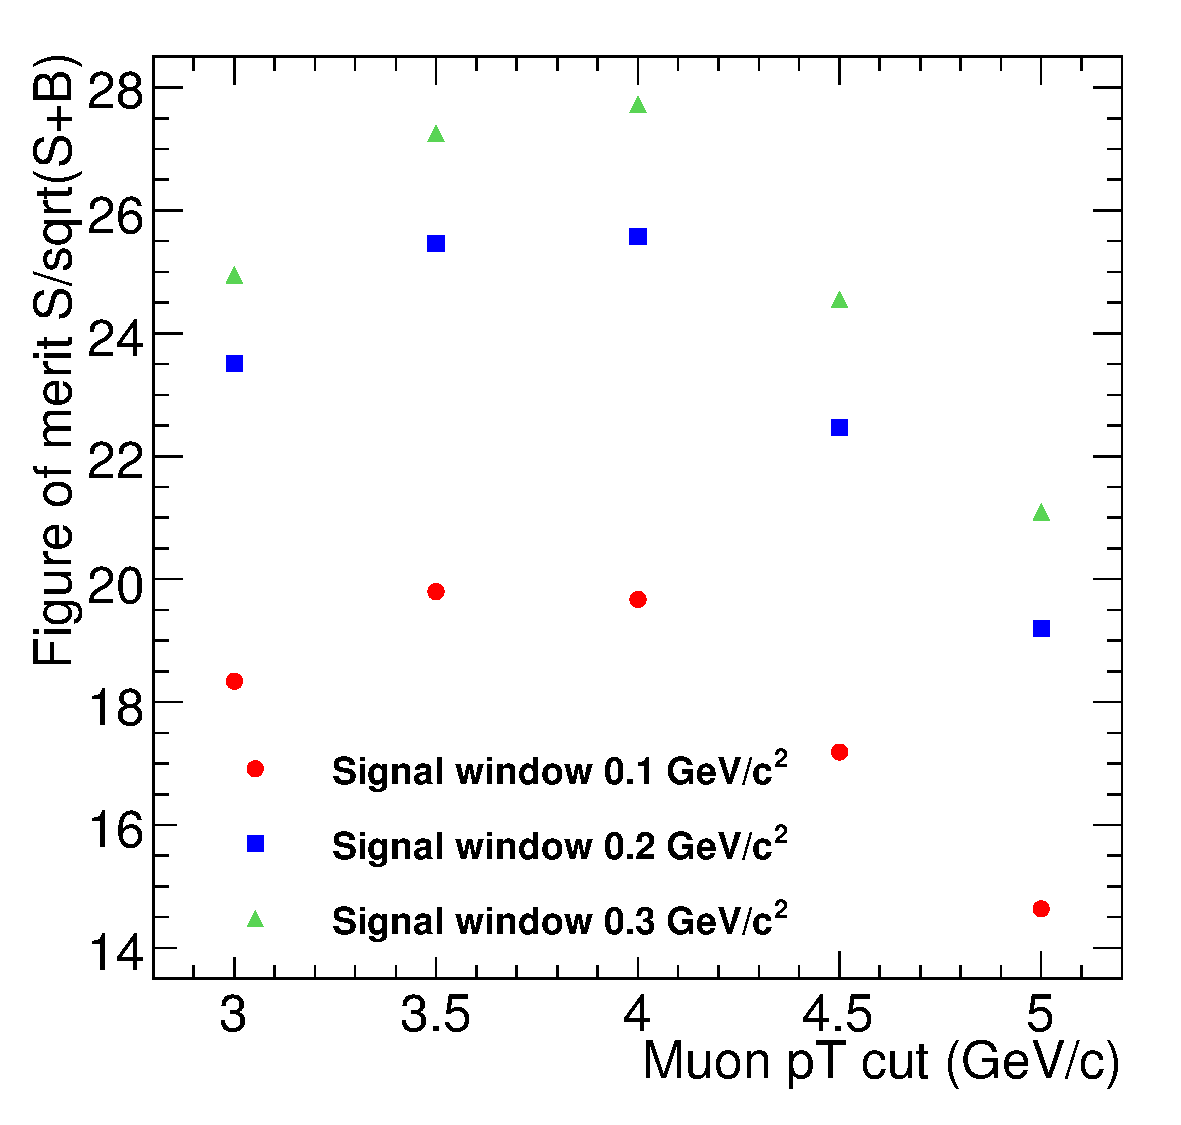
\includegraphics[angle=0,width=0.6\textwidth]{chap_YInPbPbColl2011_figures/MuonPtFom1}
    \caption{Significance of $\Upsilon(1S)$ peak as a function of the single muon $p_T$ cut}
    \label{fig:mu_pt_significance}
 \end{center}
\end{figure}

It is important to note that this optimization procedure finds the single muon $\pt$ cut giving the most significant $\PgUa$ yield. As one of the main goals of this analysis is the measurement of the relative suppression of $\PgU$ excited states with respect to the ground state and pp reference, alternative figures of merit are further investigated. It should be further noted that systematic effects are not accounted for in the procedure.  


\subsubsection{Background shape sculpting}

In the selection of the single muon $\pt$ cut, the dependence on the shape of the background should be also considered. 
These effects may be conveniently estimated by inspecting the invariant mass spectrum of the same-sign muon pairs. 
%was taken as an approximation of the background shape. 
Figure~\ref{fig:mu_pt_bkg_shape} shows the same-sign muon-pairs mass spectra, in the vicinity of the $\PgU(nS)$ mass region, obtained with different $\pt^\mu$ cut thresholds. The $\PgU(nS)$ signal nominal masses are: 9.46 \GeVcc (1S), 10.02 \GeVcc (2S), 10.36 \GeVcc (3S).  
In all cases, a peaking background distribution is expected, within the nominal fitting range; the mass value where the maximum occurs increases with the increasing $\pt$ cut.
%
\begin{figure}[h!]
 \begin{center}
    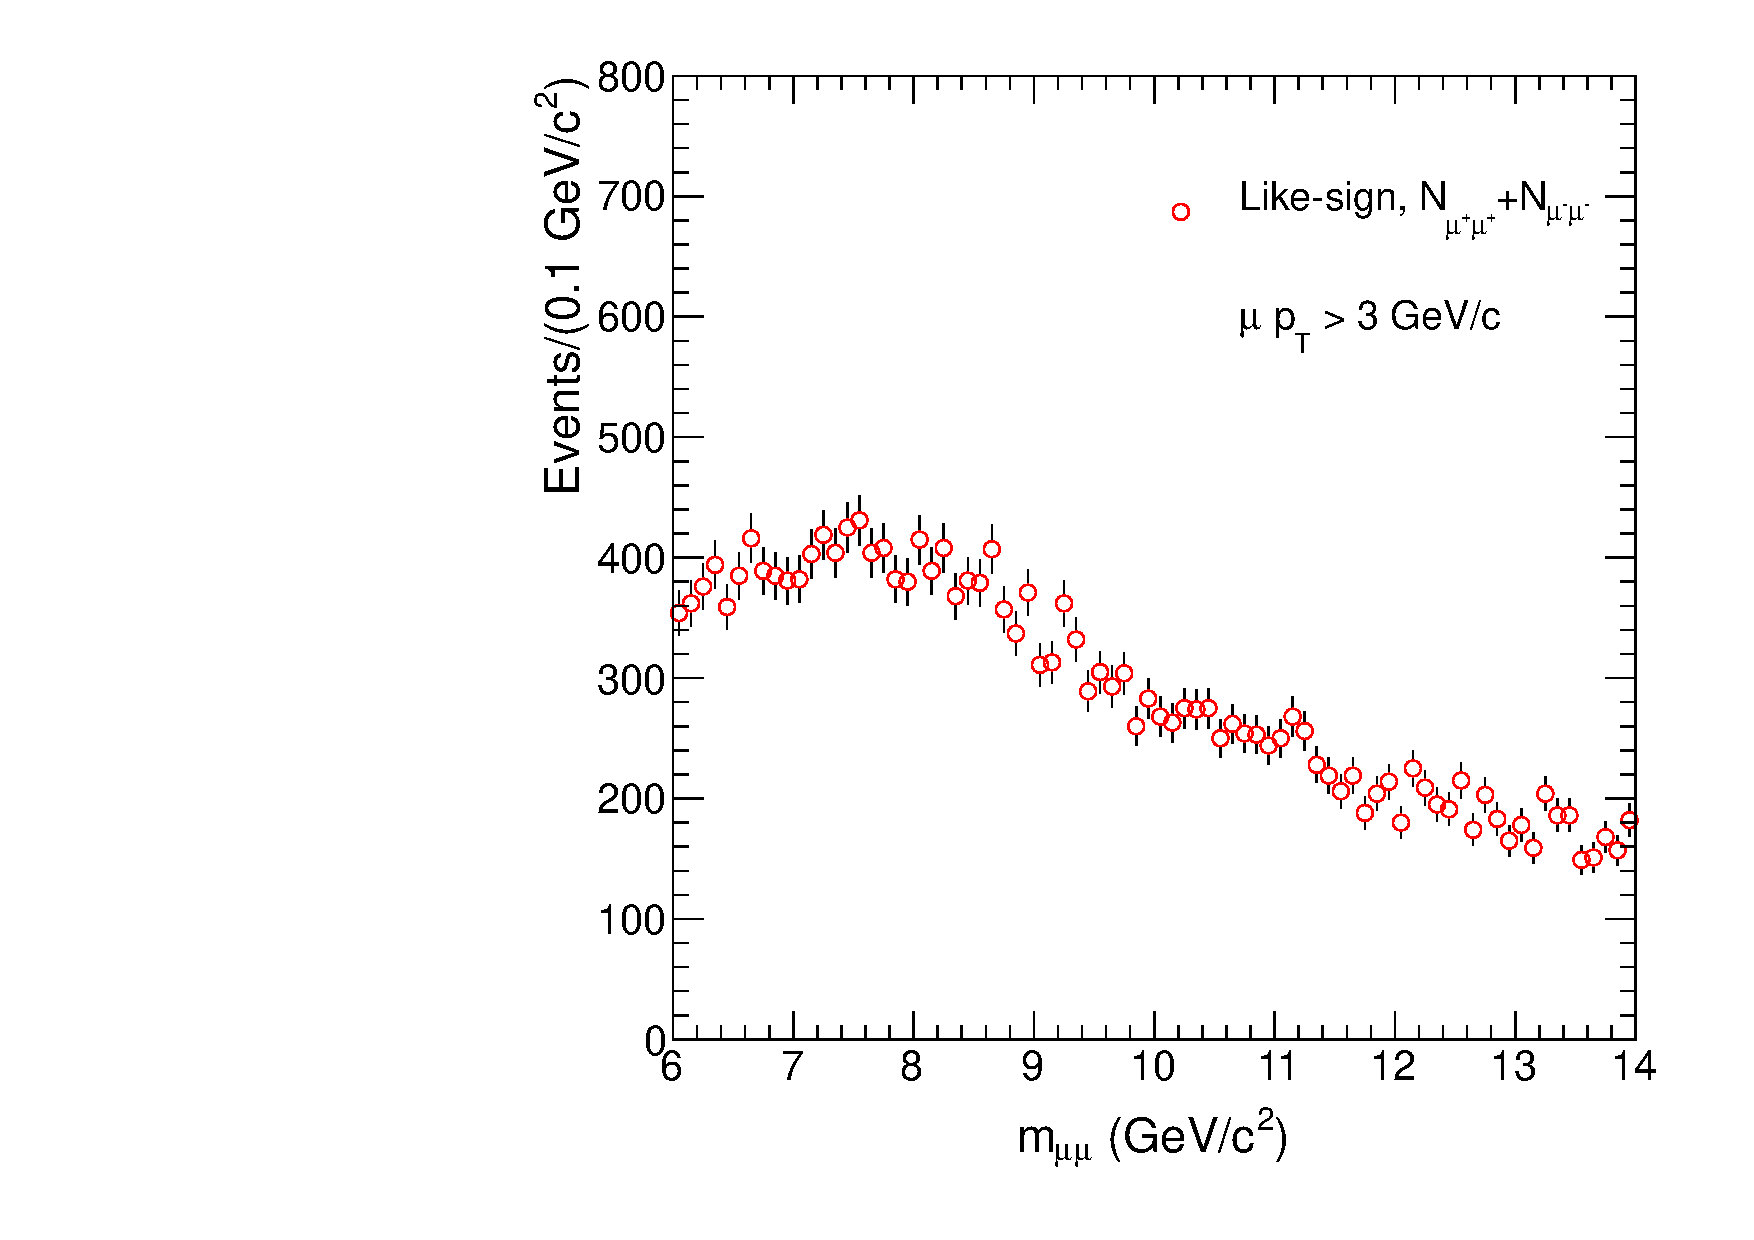
\includegraphics[angle=0,width=0.45\textwidth]{chap_YInPbPbColl2011_figures/dimuon_likesign_pt3}
    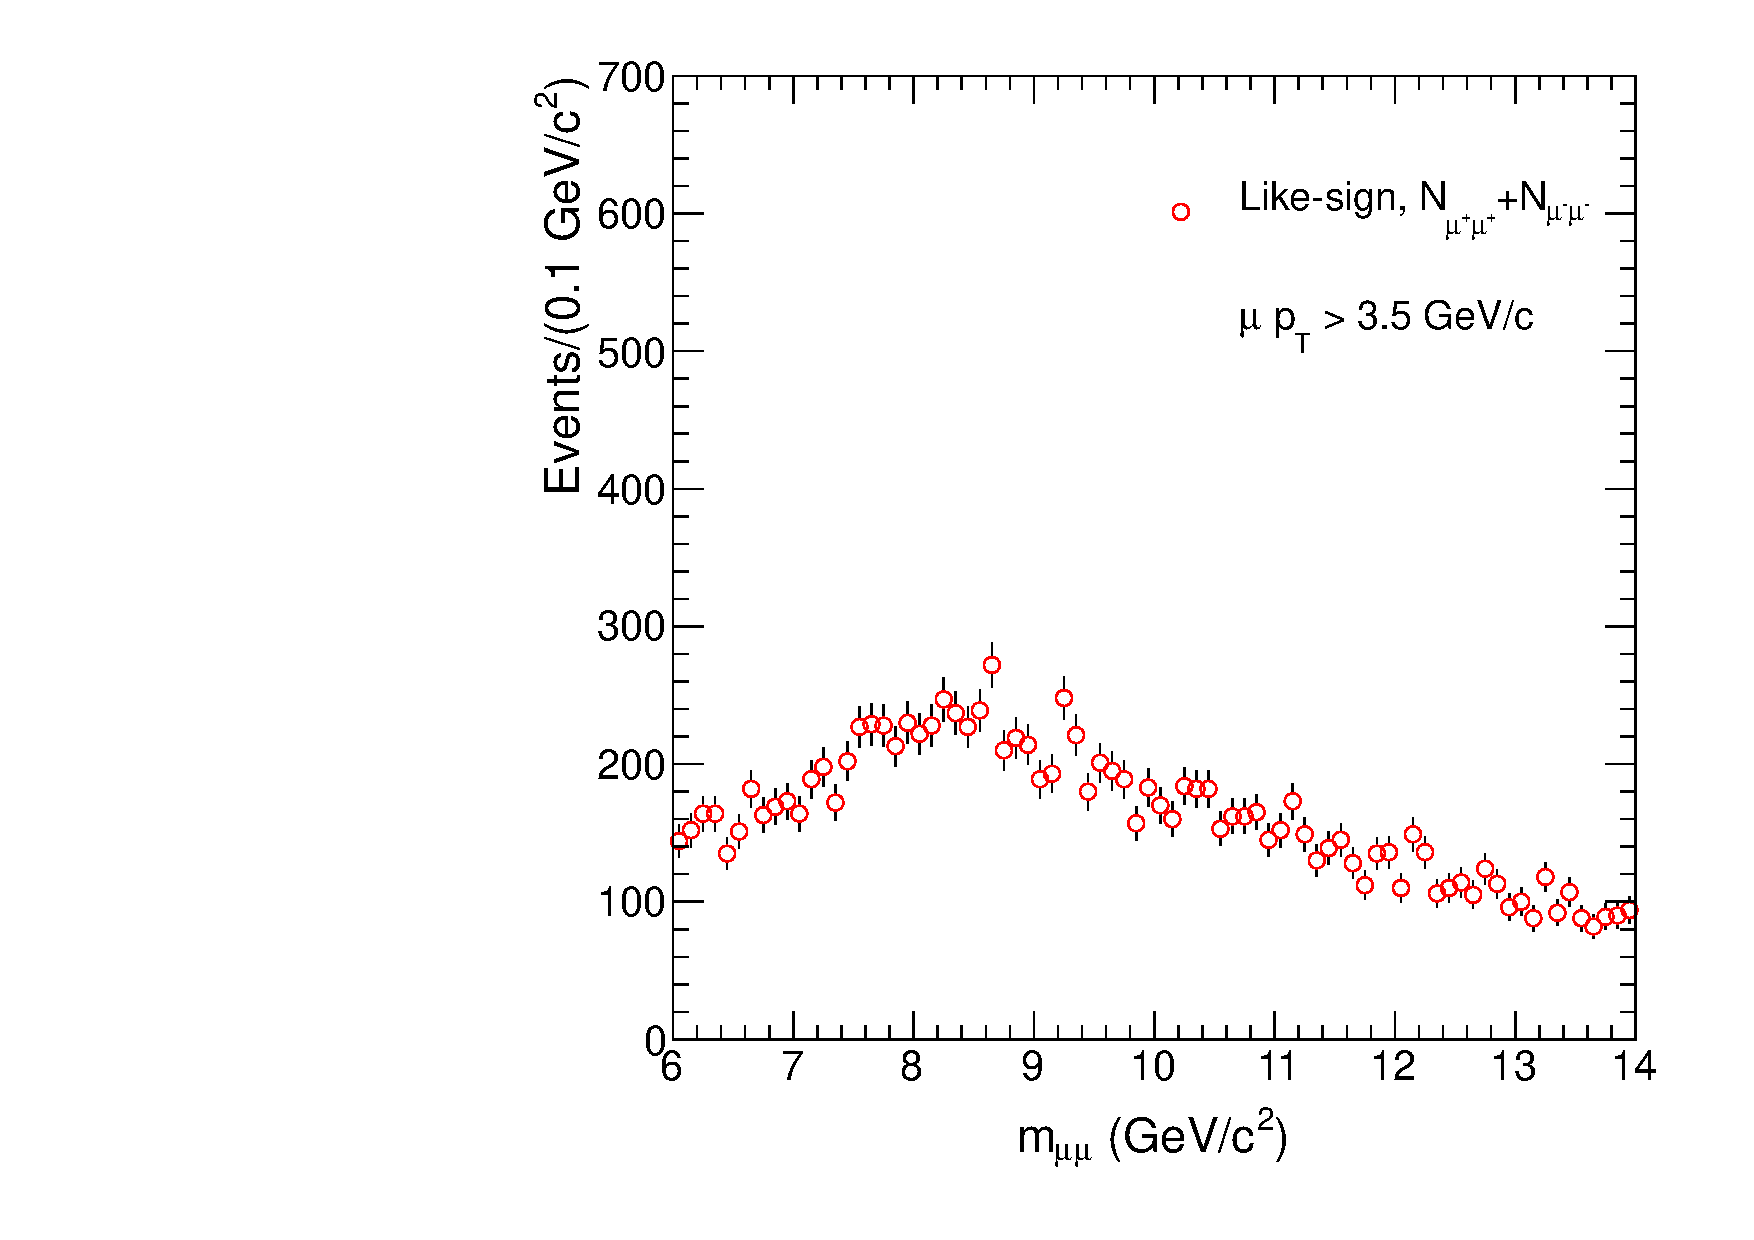
\includegraphics[angle=0,width=0.45\textwidth]{chap_YInPbPbColl2011_figures/dimuon_likesign_pt35}\\
    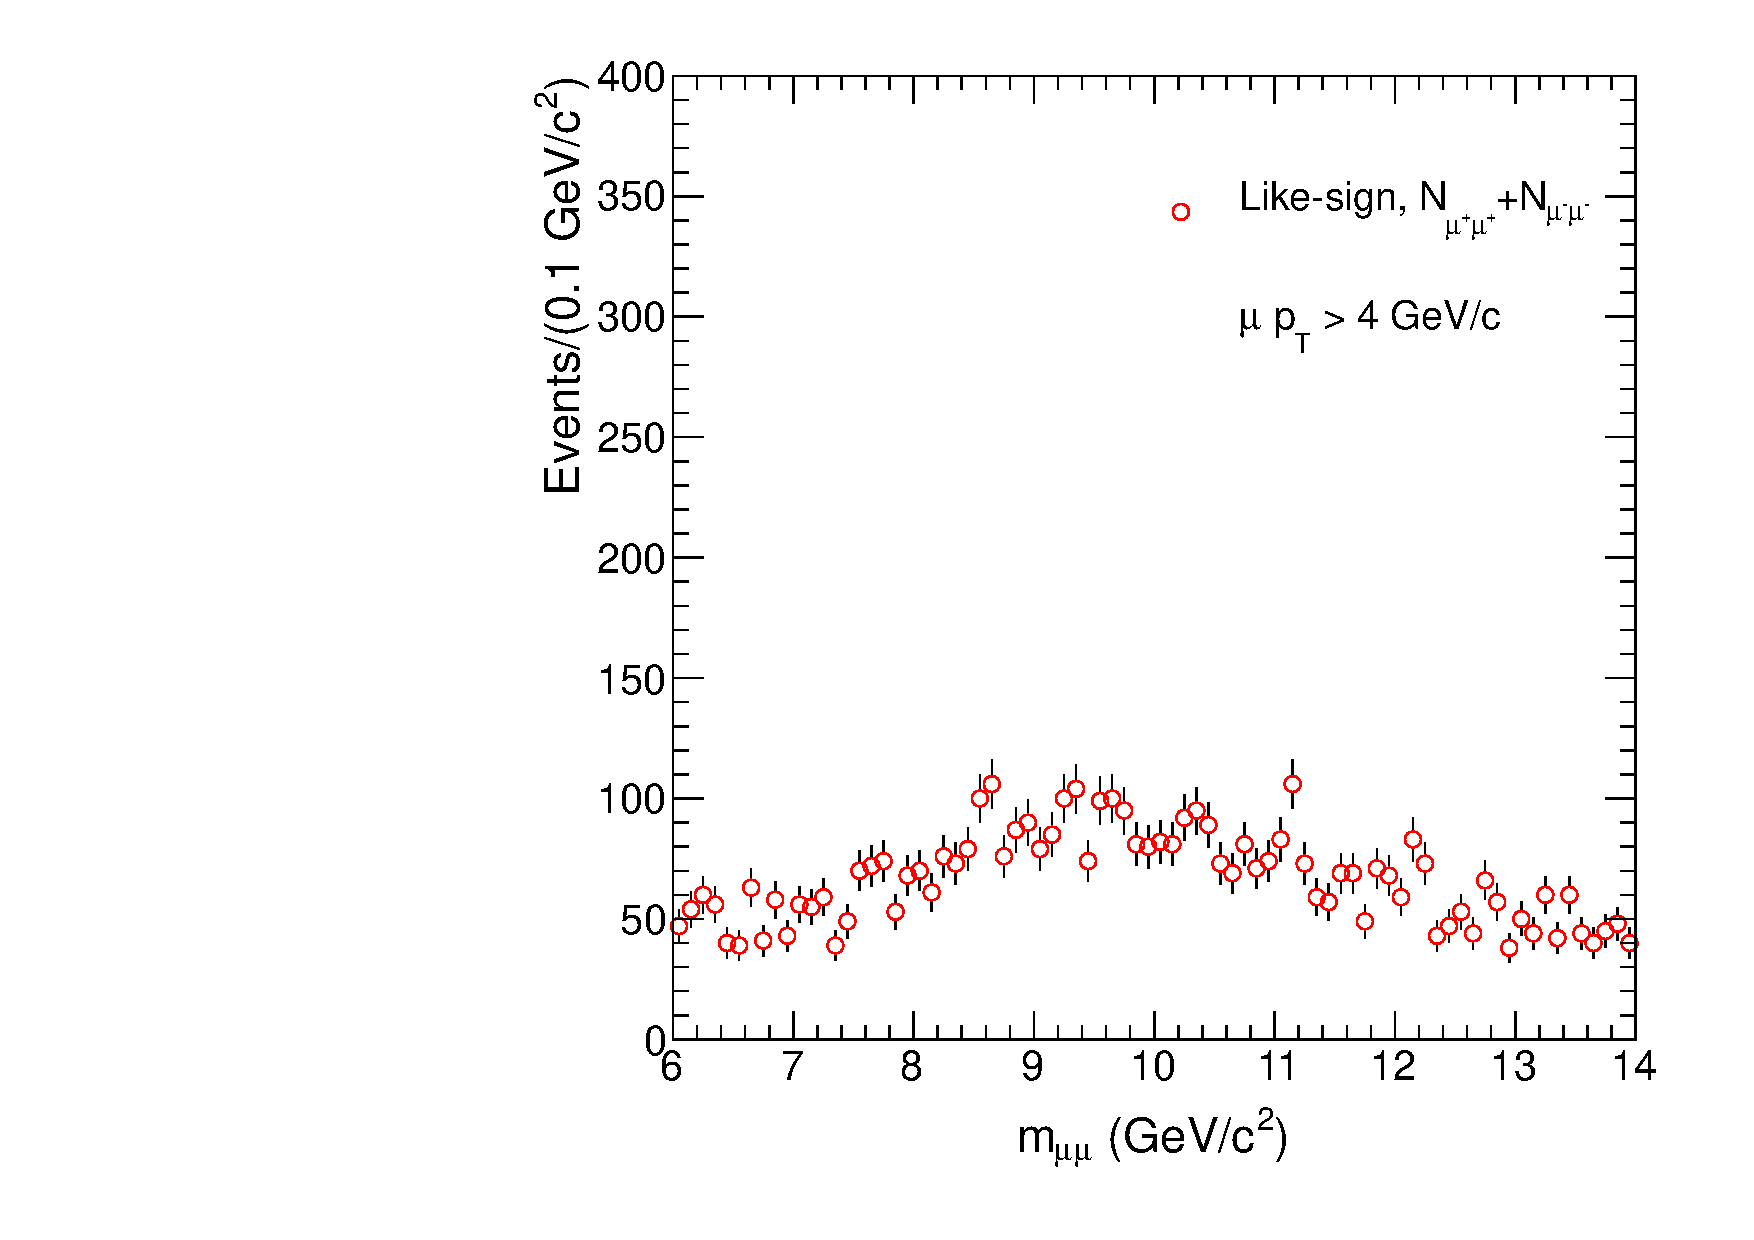
\includegraphics[angle=0,width=0.45\textwidth]{chap_YInPbPbColl2011_figures/dimuon_likesign_pt4}
    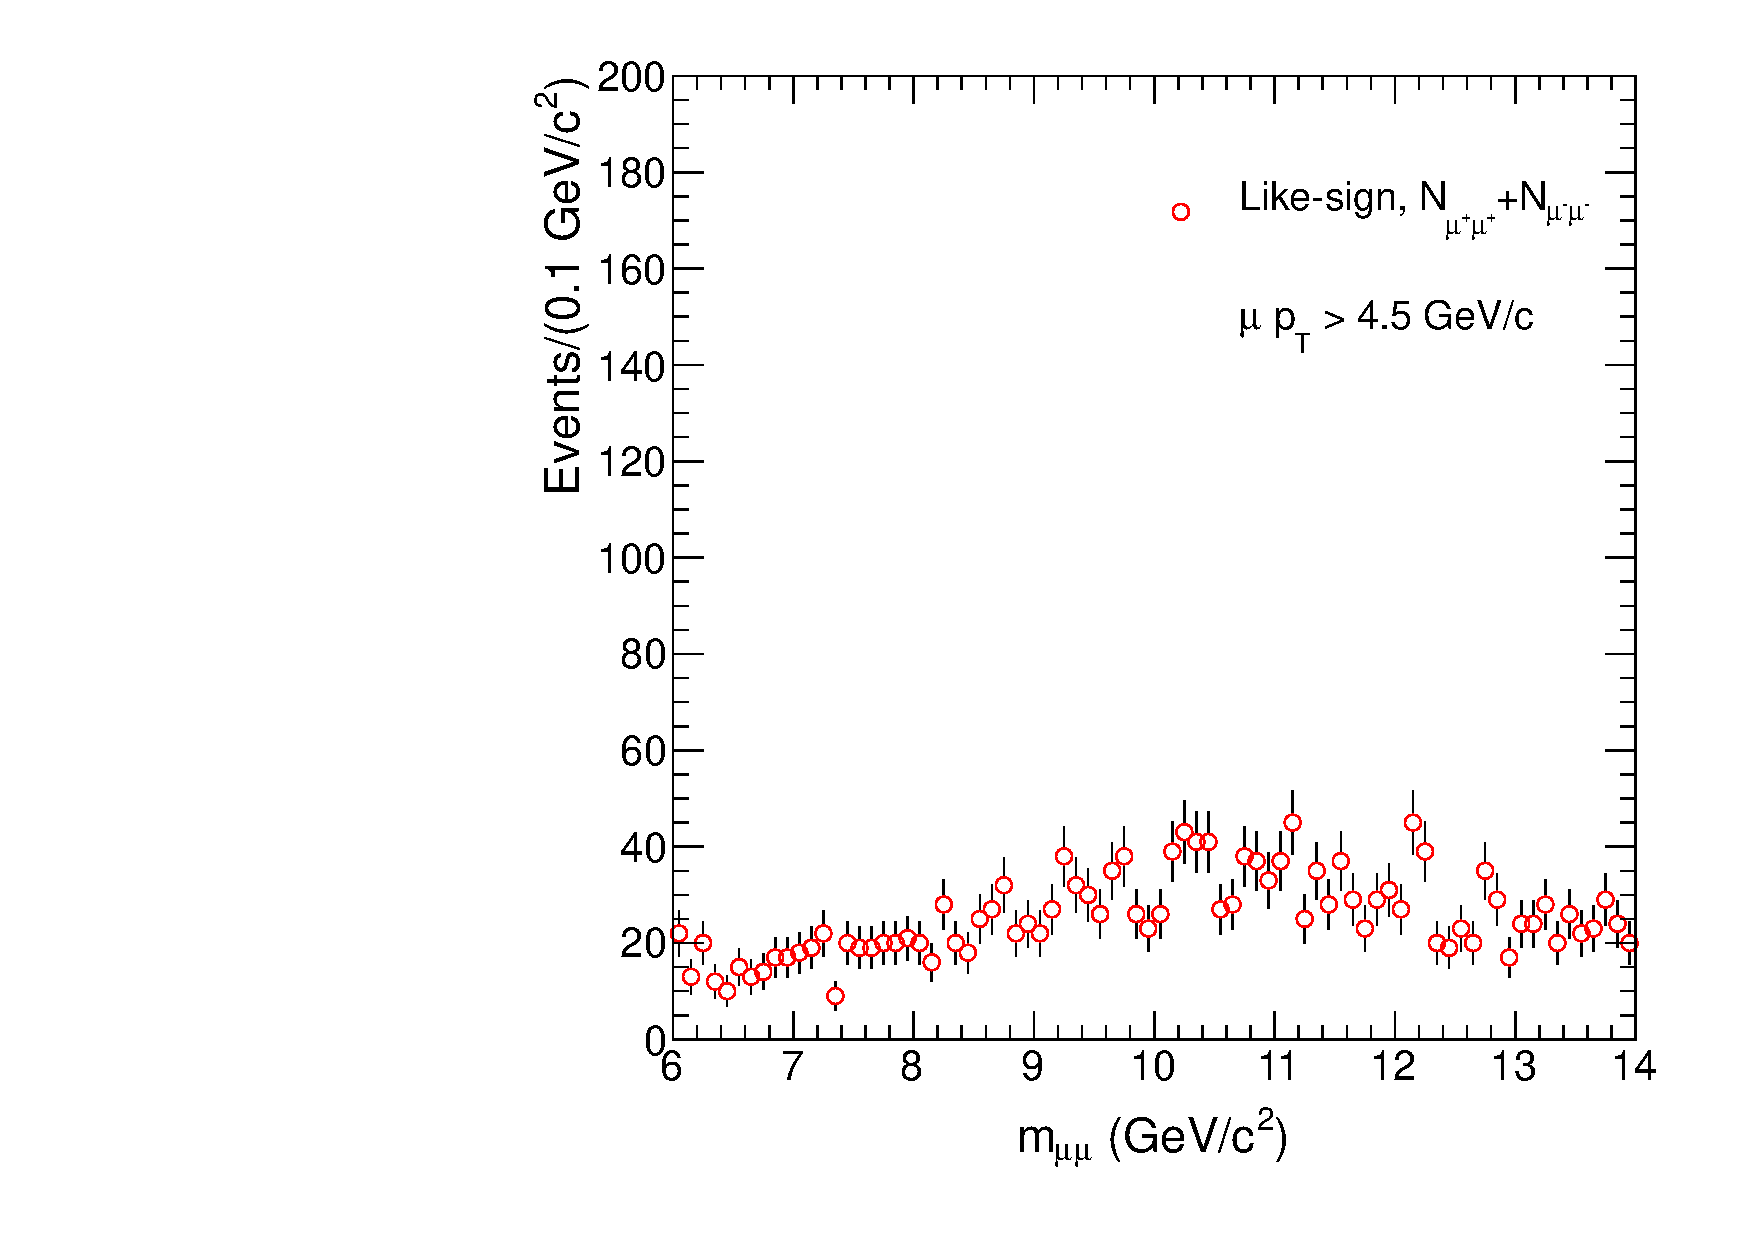
\includegraphics[angle=0,width=0.45\textwidth]{chap_YInPbPbColl2011_figures/dimuon_likesign_pt45}
    \caption{Same-sign muon pairs invariant mass distribution with different muon $\pt$ cuts, shown in the vicinity of the $\PgU(nS)$ mass region.}
    \label{fig:mu_pt_bkg_shape}
 \end{center}
\end{figure}

In the previous analysis~\cite{prl}, the cut $\pt>4 \GeVc$ was chosen. 
In this case, the background displays a peak hight underneath the $\PgU$(nS) signal mass region.
% which gives a great uncertainty on the fit results.
This results in a potentially larger systematic uncertainty associated to the background shape. 

In case of the $\pt>3.5$~\GeVc cut, %favored by the optimization described above, 
the peak in the background spectrum is located to the left of the $\PgU$ signal region. 
This should allow a better constraint by the fitter of the background shape under the signal peaks.   %gives a strong argument in 
This argument therefore favors the 3.5~\GeVc cut.

The $\pt$ cut dependence 
%of the QCD background 
of the combinatorial background shape 
was studied also in pp collisions at $\sqrt{s}=7$~TeV in data and simulation~\cite{site-bgshoulder}.  
A very similar trend is observed in pp collisions with much higher statistics. The kinematic cut removes a large portion of the background in the lower mass region and produces a step-like shape. For the case of the $\pt>3.5$~\GeVc cut, this shape is located to the left of the $\PgU$ signals; in case of $\pt>4$~\GeVc cut, it occurs instead well within the signal region, which leads to potential increases of the fit procedure uncertainties.


\subsubsection{Alternative figures of merit}
\label{AlternativeFOMs}

Alternative figures of merit were also investigated which aim at optimizing the precision of the ratio measurement (instead of the 1S peak significance). 

The first alternative method attempts to minimize the uncertainty on the ratio $N(\PgUb+\PgUc)/N(\PgUa)$, where the ratio is approximately estimated as $2B/(S+B)$. %As in the previous sections, 
$S$ is the signal counted from the MC $\PgUa$ peak and $B$ is the background in the signal window determined from the data sidebands assuming a linear mass shape. % as a function of the mass. 
The $2S$ and $3S$ peaks are approximated by the background hypothesis, that is, assuming the background level overwhelms the signal, which is approximately the case.
To normalize the background from data and signal from MC together, the 1S peak in data is fitted and the integral in the given signal window is used as normalization factor.

The uncertainty on the ratio to be minimized is $\frac{2B}{S+B}\sqrt{\frac{1}{2B}+\frac{1}{S+B}}$, as calculated with standard error propagation and using  $\sqrt{S}$ and $\sqrt{B}$ as estimates for the uncertainties on $S$ and $B$.  
%
The results of the calculation are shown in Fig.~\ref{fig:mu_pt_ratio}, for three different values of the signal mass window size. The points reach a minimum at single muon $\pt>4$~\GeVc independent of the size of the signal window. This optimization method favors a \pt{} cut value at 4~\GeVc.

\begin{figure}[h!]
 \begin{center}
    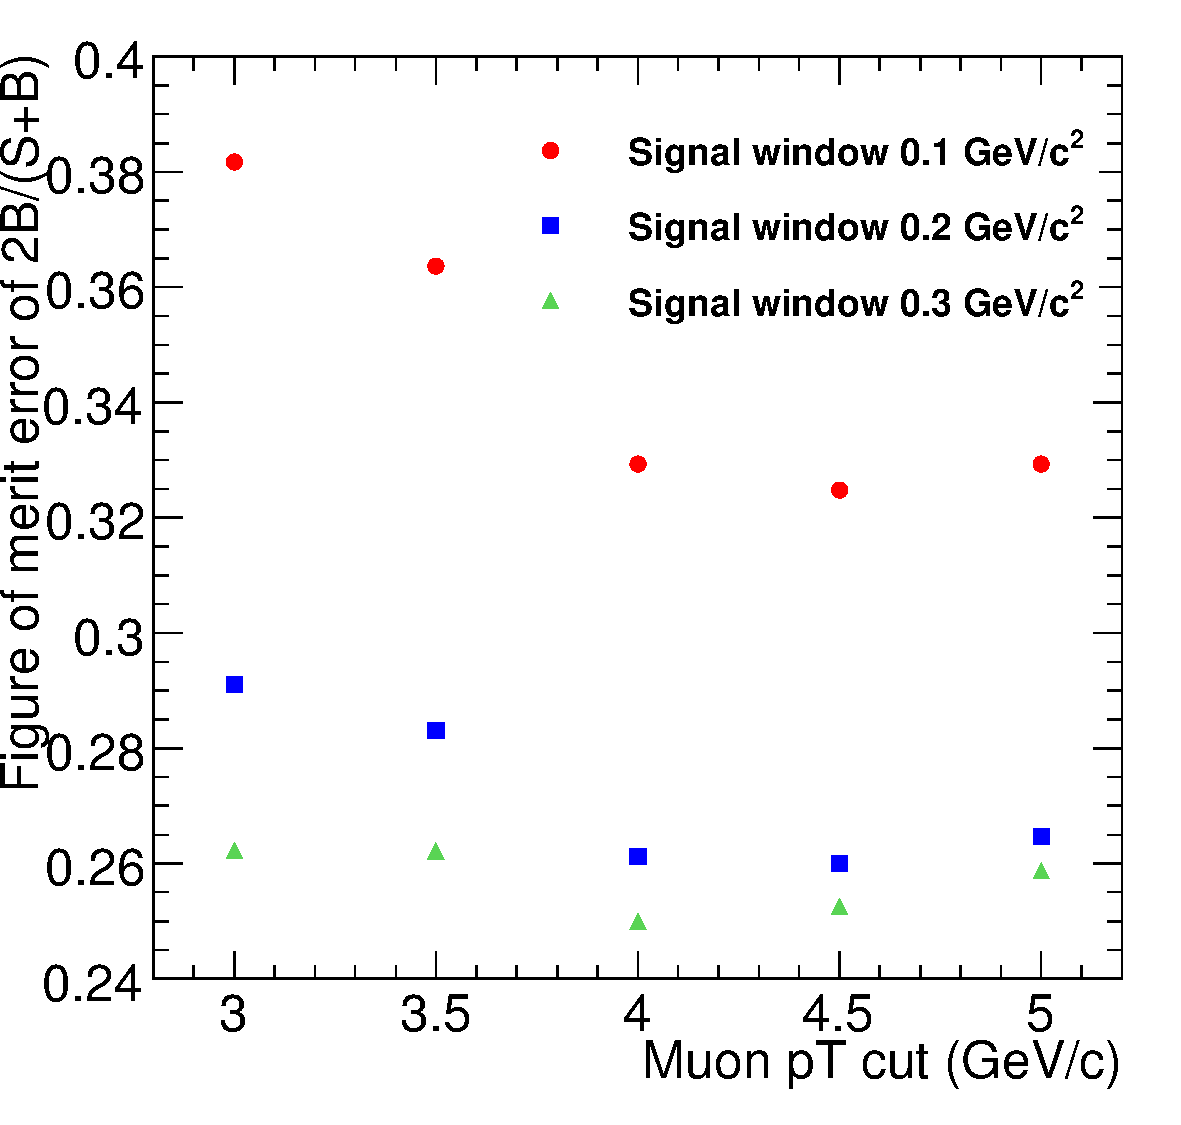
\includegraphics[angle=0,width=0.6\textwidth]{chap_YInPbPbColl2011_figures/MuonPtFom2}
    \caption{Uncertainty on the $2B/(S+B)$ quantity as a function of the single muon $\pt$ cut.}
    \label{fig:mu_pt_ratio}
 \end{center}
\end{figure}

%It is important to note that minimizing the uncertainty of the measured quantity could potentially indirectly bias the outcome of the measurement. 
%
A third optimization method has also been explored, where we attempt to assess the expected sensitivity on the double ratio directly, by employing pseudo-experiments, generated according to fits performed to the data after each cut.
%
The procedure is as follows. We fit the data sample and then generate 10000 toy MC pseudo-data according to parameters in the covariant matrix from the fitting. The double ratio of \PbPb/\pp is generated at unity in the pseudo-data. The statistics of each sample is fixed to the amount of data we observe. These toys represent the outcome of many CMS experiments assuming nature had no upsilon excited state suppression. We plot the distribution of the ratio parameter, $\chi$, measured in each toy experiment. We find the $p$-value (see Section~\ref{sec:signficance}) associated to a reference $\chi-0.5$ value. We repeat the same steps for different selection cuts and identify the best cut the one resulting in the smallest $p$-value. 

The plots for two different single muon transverse momentum thresholds, $\pt^\mu>3.5\GeVc$ and $\pt^\mu>4.0\GeVc$, are shown in \fig{fig:toy_nullhypo}.
%
The reach of the two cuts is similar with the tighter cut yielding a smaller $p$-value. 
This is likely due to the signal to background ratio being better with the tighter cut. 
However, relevant systematic effects have not been included in the pseudo-experiments study.

\subsubsection{\PgUa signal \pt}
If we define the \PgUa signal region as (9.2, 9.8), the side-band region as (8, 8.5) and (12, 14), we can plot the signal events \pt distribution, side-band events \pt distribution, and side-band subtracted events \pt distribution, as shown in \fig{fig:upsPt}. The \PgUa signal mean \pt is 5.9\GeVc after side-band subtraction.
\begin{figure}[h!]
 \begin{center}
   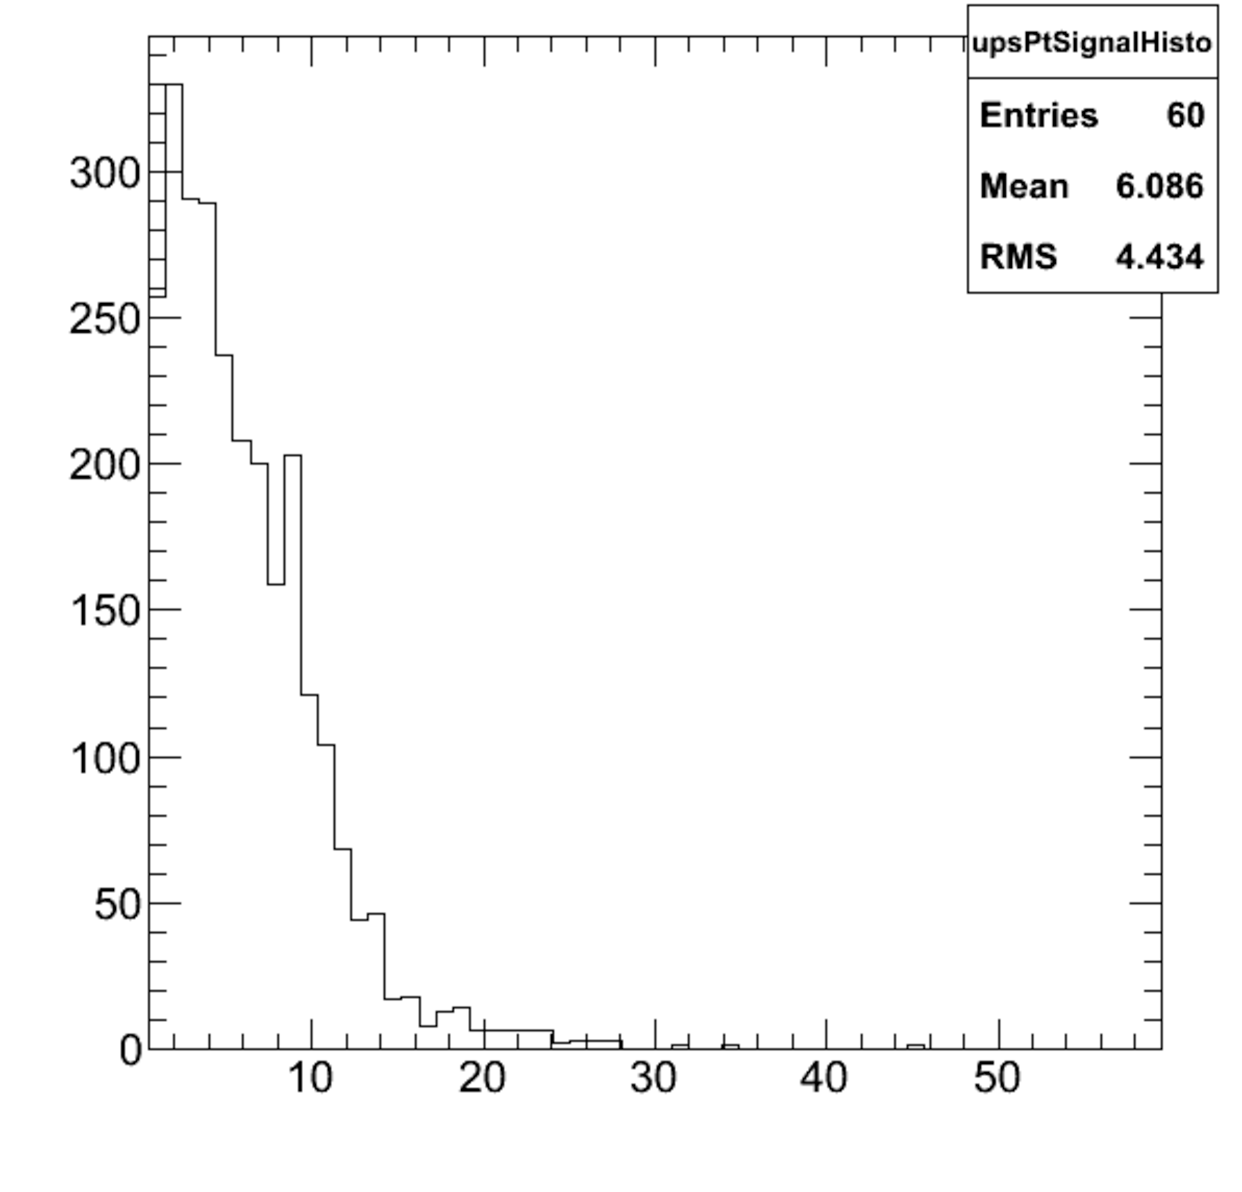
\includegraphics[angle=0,width=0.33\textwidth]{chap_YInPbPbColl2011_figures/upsPtSignalHisto}
   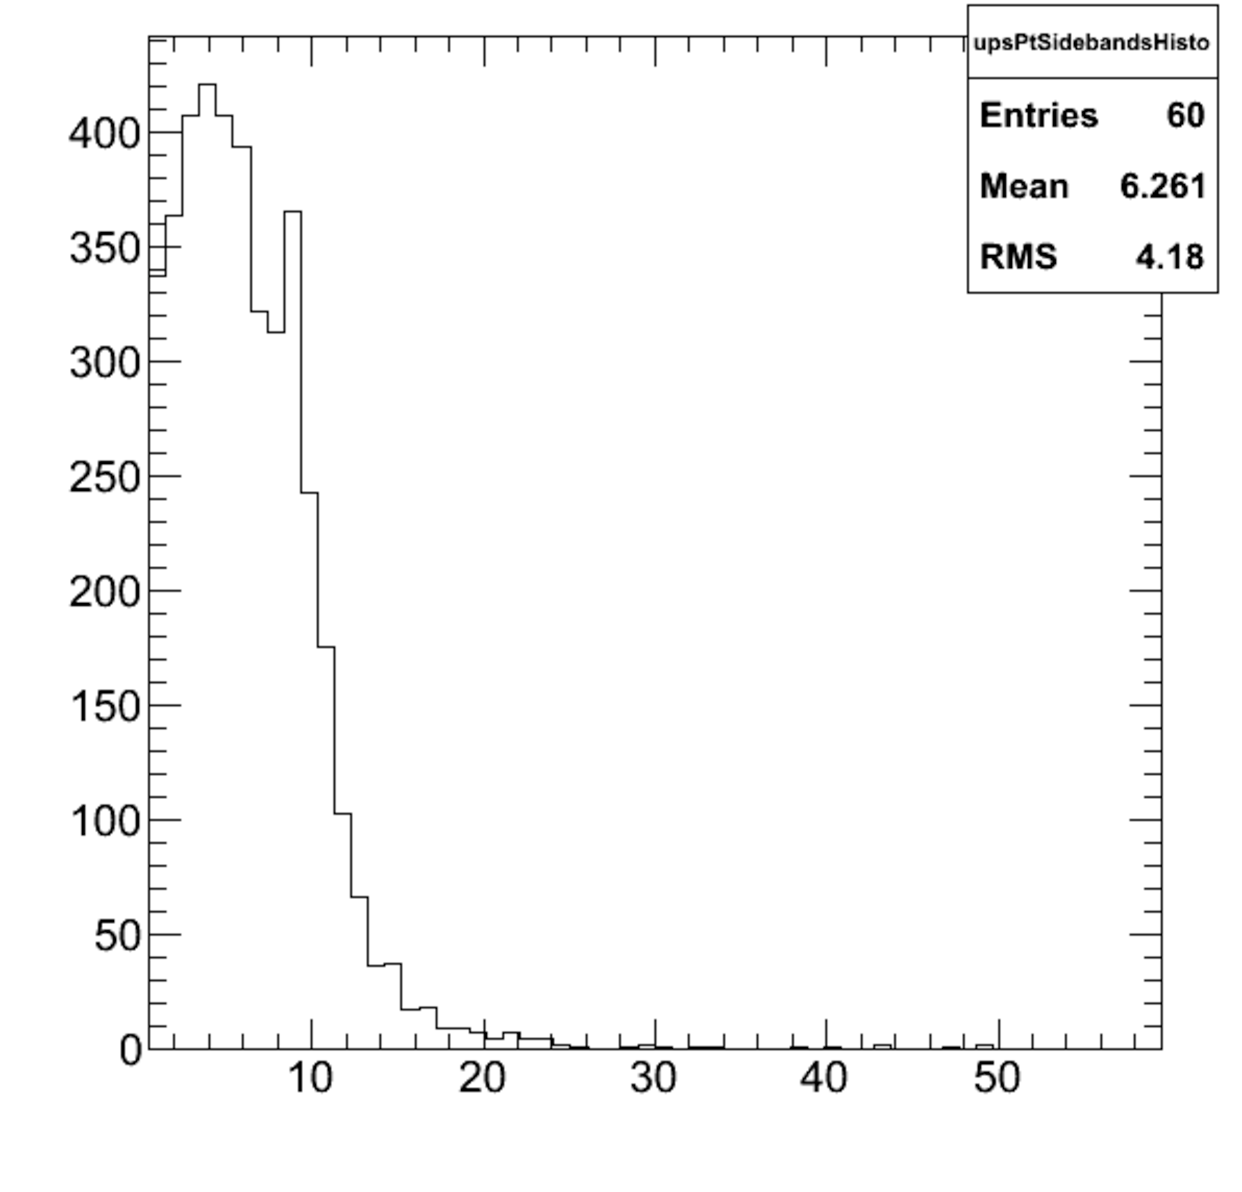
\includegraphics[angle=0,width=0.33\textwidth]{chap_YInPbPbColl2011_figures/upsPtSidebandsHisto}
   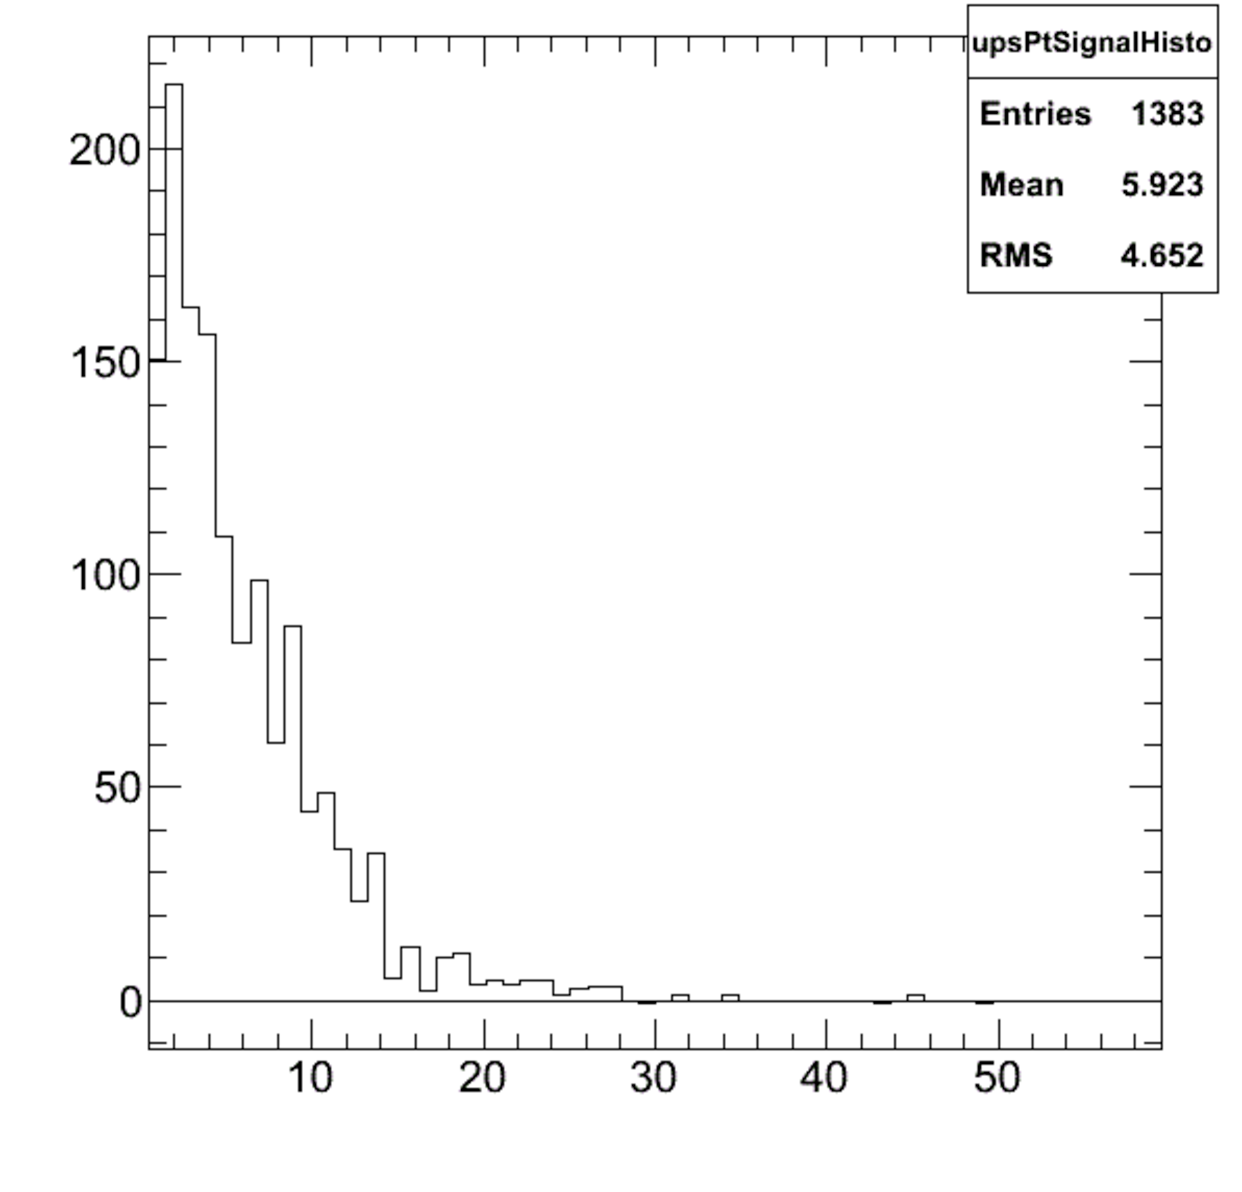
\includegraphics[angle=0,width=0.33\textwidth]{chap_YInPbPbColl2011_figures/upsPtSubtracted}
   \caption{\PgUa \pt distributions} %(default {\tt 1\%).}} 
   \label{fig:upsPt}
 \end{center}
\end{figure}


\subsection{Summary of offline selection}

In order to select good quality muons the effect of different cut thresholds on a variable set was studied. 
%Table~ below summarizes the effect of the cuts chosen. 
%Applying all the cuts keeps between about 90\% of the signal depending. 
%The background rejection is estimated to be about 30\%. 
%Requiring the number of inner tracker hit to be higher than 10 together with the muon arbitration cut have the biggest impact on the background rejection.
Table~\ref{tab:Efficiency_cuts_all} shows the effect on the significance, as well as signal efficiency and background rejection, when applying all other cuts but the one studied. %, on MC and data. 
It further gives an indication of the correlation between the cuts. 
Once the nominal cut thresholds are applied, variations of a single cut have little impact on the significance. 
%The arbitration cut is the one that removes the most background in the data. -- this is not shown in the study performed here!!
\begin{table}[h!]
\begin{center}  
\caption{Estimated $\PgUa$ yield significance, signal efficiency (MC) and background rejection in \% after applying all other cuts but the one listed.}
   \vspace{1em}
  \label{tab:Efficiency_cuts_all}
\begin{tabular}{c|c|c|c}
\hline
Cut Variable   &real data                   &MC                     &Significance \\ 
               &1-$\epsilon_{Bkg}$[\%]       &$\epsilon_{Bkg}$[\%]     & \\
\hline
 InnerTrackHits $>$ 10                       &51.0 &85.0 &14.5 \\  
 PixeLayers       $>$ 0                      &54.1  &84.6  &14.6 \\
 InnerTrack$\chi^2/ndf<$4.                   &53.2  &84.7  &14.5 \\
 Dxy    $<$ 3. cm                            &54.1  &84.6  &14.6 \\
 Dz       $<$ 15.  cm                        &54.1  &84.6  &14.6 \\
 GlobalTrack$\chi^2/ndf<$20                  &51.8  &87.2  &15.1 \\
 vProb $>$ 0.05                              &20.2  &89.5  &13.7\\ 
 TrackerMuonArbitrated =1                    &52.7  &84.9  &14.5\\ \hline
 All cuts                                    &54.1  &84.6  &14.6\\ \hline
\end{tabular}
\end{center}
\end{table}


In order to select muons in the acceptance and reject the background while keeping as much signal as possible a single muon $\pt$ cut is introduced. 
The choice of the muon \pt cut value involves various considerations. 
The nominal cut is chosen to be $\pt>4.0$~\GeVc, which was also used in the previous analysis iteration~\cite{prl}.
This is supported by the outcome of the statistical optimization procedure, employing different heuristic figures of merit; in addition, 
the systematic effect due to the kinematic background may be controlled, as discussed in Sec.~\ref{sec:bgmodel}. 
The argument to support it is the significance study performed on the $\PgU(1S)$ peak that shows a maximum at $4.0$~\GeVc.
The second argument, perhaps even stronger than the first one, is the background shape variation due to the muon $\pt$ cut. 

%While it rejects more background, the background shape shows in this case a peaking structure whithin the $\PgU$ signal mass 
%region (ie, underneath the signal peaks), leading to a potetnial increase of the systematic uncertainty associated to the fitting procedure. 
%This peak in the background shape moves to lower masses (ie, further to the left and away from the signal peaks) once a lower cut is chosen. 



